%%%%%%%%%%%%%%%%%%%%%%%%%%%%%%%%%%%%%%%%%%%%%%%%%%%%%%%%%%%%%%%%%%%%%%%
%% template for II2202 report
%% original 2015.11.24
%% revised  2016.08.23
%%%%%%%%%%%%%%%%%%%%%%%%%%%%%%%%%%%%%%%%%%%%%%%%%%%%%%%%%%%%%%%%%%%%%%%
%

\title{Designing Deixis Usage in Real-time Collaborative Drawing}
\author{
        \textsc{Jiayao Yu}
            \qquad
        \textsc{Yumin Hong}
        \mbox{}\\
        \normalsize
            \texttt{jiayaoy}
        \textbar{}
            \texttt{yumin}
        \normalsize
            \texttt{@kth.se}
}
\date{\today}

\documentclass[12pt,twoside]{article}

\usepackage[paper=a4paper,dvips,top=1.5cm,left=1.5cm,right=1.5cm,
    foot=1cm,bottom=1.5cm]{geometry}
\usepackage{booktabs}

%\usepackage[T1]{fontenc}
%%\usepackage{pslatex}
\renewcommand{\rmdefault}{ptm} 
\usepackage{mathptmx}
\usepackage[scaled=.90]{helvet}
\usepackage{courier}
%
\usepackage{bookmark}

\usepackage{fancyhdr}
\pagestyle{fancy}

%%----------------------------------------------------------------------------
%%   pcap2tex stuff
%%----------------------------------------------------------------------------
 \usepackage[dvipsnames*,svgnames]{xcolor} %% For extended colors
 \usepackage{tikz}
 \usetikzlibrary{arrows,decorations.pathmorphing,backgrounds,fit,positioning,calc,shapes}

%% \usepackage{pgfmath}	% --math engine
%%----------------------------------------------------------------------------
%% \usepackage[latin1]{inputenc}
\usepackage[utf8]{inputenc} % inputenc allows the user to input accented characters directly from the keyboard
\usepackage[swedish,english]{babel}
%% \usepackage{rotating}		 %% For text rotating
\usepackage{array}			 %% For table wrapping
\usepackage{graphicx}	                 %% Support for images
\usepackage{float}			 %% Suppor for more flexible floating box positioning
\usepackage{color}                       %% Support for colour 
\usepackage{mdwlist}
%% \usepackage{setspace}                 %% For fine-grained control over line spacing
%% \usepackage{listings}		 %% For source code listing
%% \usepackage{bytefield}                %% For packet drawings
\usepackage{tabularx}		         %% For simple table stretching
%%\usepackage{multirow}	                 %% Support for multirow colums in tables
\usepackage{dcolumn}	                 %% Support for decimal point alignment in tables
\usepackage{url}	                 %% Support for breaking URLs
\usepackage[perpage,para,symbol]{footmisc} %% use symbols to ``number'' footnotes and reset which symbol is used first on each page

%% \usepackage{pygmentize}           %% required to use minted -- see python-pygments - Pygments is a Syntax Highlighting Package written in Python
%% \usepackage{minted}		     %% For source code highlighting

%% \usepackage{hyperref}		
\usepackage[all]{hypcap}	 %% Prevents an issue related to hyperref and caption linking
%% setup hyperref to use the darkblue color on links
%% \hypersetup{colorlinks,breaklinks,
%%             linkcolor=darkblue,urlcolor=darkblue,
%%             anchorcolor=darkblue,citecolor=darkblue}

%% Some definitions of used colors
\definecolor{darkblue}{rgb}{0.0,0.0,0.3} %% define a color called darkblue
\definecolor{darkred}{rgb}{0.4,0.0,0.0}
\definecolor{red}{rgb}{0.7,0.0,0.0}
\definecolor{lightgrey}{rgb}{0.8,0.8,0.8} 
\definecolor{grey}{rgb}{0.6,0.6,0.6}
\definecolor{darkgrey}{rgb}{0.4,0.4,0.4}
%% Reduce hyphenation as much as possible
\hyphenpenalty=15000 
\tolerance=1000

%% useful redefinitions to use with tables
\newcommand{\rr}{\raggedright} %% raggedright command redefinition
\newcommand{\rl}{\raggedleft} %% raggedleft command redefinition
\newcommand{\tn}{\tabularnewline} %% tabularnewline command redefinition

%% definition of new command for bytefield package
\newcommand{\colorbitbox}[3]{%
	\rlap{\bitbox{#2}{\color{#1}\rule{\width}{\height}}}%
	\bitbox{#2}{#3}}

%% command to ease switching to red color text
\newcommand{\red}{\color{red}}
%%redefinition of paragraph command to insert a breakline after it
\makeatletter
\renewcommand\paragraph{\@startsection{paragraph}{4}{\z@}%
  {-3.25ex\@plus -1ex \@minus -.2ex}%
  {1.5ex \@plus .2ex}%
  {\normalfont\normalsize\bfseries}}
\makeatother

%%redefinition of subparagraph command to insert a breakline after it
\makeatletter
\renewcommand\subparagraph{\@startsection{subparagraph}{5}{\z@}%
  {-3.25ex\@plus -1ex \@minus -.2ex}%
  {1.5ex \@plus .2ex}%
  {\normalfont\normalsize\bfseries}}
\makeatother

\setcounter{tocdepth}{3}	%% 3 depth levels in TOC
\setcounter{secnumdepth}{5}
%%%%%%%%%%%%%%%%%%%%%%%%%%%%%%%%%%%%%%%%%%%%%%%%%%%%%%%%%%%%%%%%%%%%
%% End of preamble
%%%%%%%%%%%%%%%%%%%%%%%%%%%%%%%%%%%%%%%%%%%%%%%%%%%%%%%%%%%%%%%%%%%%

\renewcommand{\headrulewidth}{0pt}
\lhead{II2202, Fall 2017, Period 1-2}
%% or \lhead{II2202, Fall 2016, Period 1}
\chead{Final project report}
\rhead{\date{\today}}

\makeatletter
\let\ps@plain\ps@fancy 
\makeatother

\setlength{\headheight}{15pt}
\begin{document}

\maketitle


\begin{abstract}
\label{sec:abstract}

Humans are used to using deixis in face-to-face collaborations during evolution over thousands of years, to facilitate communication by shortening and simplifying dialogue. However, in geographically separated Computer-Supported Cooperative Work (CSCW), it is awkward to use deixis due to lack of contextual information. In this paper, we focused on real-time collaborative drawing, analyzed deixis usage in face-to-face collaboration and CSCW respectively based on our field experiment and exploratory data analysis. In the end we proposed an interaction design concept to optimize deixis usage in real-time collaborative drawing, with scalability to general CSCW groupware interaction designs. 
\\
\\
\textbf{Keywords}: deixis; collaborative drawing; CSCW; interaction design.

\end{abstract}

%%\clearpage

\selectlanguage{english}
\tableofcontents

% \section*{List of Acronyms and Abbreviations}
% \label{list-of-acronyms-and-abbreviations}

% This document requires readers to be familiar with terms and concepts described in \mbox{RFC~1235} \cite{john_ioannidis_coherent_1991}. For clarity we summarize some of these terms and give a short description of them before presenting them in next sections.

% \begin{basedescript}{\desclabelstyle{\pushlabel}\desclabelwidth{10em}}
% \item[IPv4]					Internet Protocol version 4 (RFC~791 \cite{postel_internet_1981})
% \item[IPv6]					Internet Protocol version 6 (RFC~2460 \cite{deering_internet_1998})
% \end{basedescript}


\clearpage
\section{Introduction}
\label{sect:introduction}
%% Longer problem statement
%% General introduction to the area

% It was conjectured in \cite{john_ioannidis_coherent_1991} that multicasting
% could provide gains by \ldots.

% See also \cite{a_new_synchronization_protocol_for_sqlite_databases},
% the paper \cite{anand_kannan_n-ary_2012}, 
% and the book \cite{brent_s._baxter_standard_1982}.

In natural face-to-face collaborations, collaborators mutually perceive information not only from explicit resulting expressions on shared media, such as writing and drawing on paper, but also from implicit accompanying indications through the collaboration process, such as facial expressions and hand gestures. To be more specific, those implicit accompanying indications are categorized as deictic words, demonstration action, and manifesting actions \cite{gutwin2002descriptive}. When collaborators refer to an object on their shared media, they often use deixis to indicate their reference. Deixis is widely used in face-to-face collaborations, while its semantic meaning is strongly dependent on situated context, which are often missing in Computer-Supported Cooperative Work (CSCW). Proper deixis usage in CSCW can help collaborators gain contextual information and facilitate their mutual communications. However, there were insufficient interaction designs for CSCW shared media groupwares to empower collaborators to use deixis as freely as face-to-face collaborations. Though there were different research frameworks on deixis usage, we still can sense the gap between theoretical research and industrial practices, especially for real-time collaborative drawing groupware designs.

In this research, we investigated how collaborators use deixis in face-to-face collaboration and CSCW by field experiment exploratory data analysis, we were able to draw five main conclusions on how and why the collaborators behave distinctly in terms of deixis usage, and derive design implications on top of them, with validations on our designs in the end.

\subsection{Background}
\label{sect:literature}
\subsubsection{Deixis}
A deixis (or deictic expression) is a word or phrase (such as this, that, these, those, now, then) that points to the time, place, or situation in which a speaker is speaking. Fillmore described this utterance situation, which includes space and time information,  as grounding in a social context \cite{fillmore1997lectures}. The term deixis was defined and classified by other scholars as well. The most accepted classification was claimed by Levinson, who divided it into person deixis, time deixis, place deixis, discourse deixis, and social deixis.

Deixis can be used in orienting addressee’s attention by situating, displacing and directing someone’s point of view. The addressee starts an orientation procedure when the speaker uses a deictic expression. Rodney and Geoffrey stated the meaning can be traced directly to features of the act of utterance, like when and where it takes place, if deixis was used in expressions\cite{huddleston2006coordination}. For Fillmore’s statement, deixis has deictic usage, and it includes gesture usage  \cite{fillmore1997lectures}, which are fully interpreted only if the speaker makes use of certain paralinguistic features such as a pointing or head moving, and the addressee is able to perceive and monitor certain aspect of the communication act. This kind of gesture usage is spontaneous. A research on gestures by 14 months old children had shown, pointing is a pre-linguistic activity with a lexical status: pointing-gestures are object-referring terms used by very young children as substitutes for words they have not yet acquired in their vocabulary \cite{goldin2007young}. Attempts at deixis in linguistics have appeared long time, but deixis research in CSCW seems limited. Therefore, insufficient applied theories urge designers to conduct user experiment as an alternative.\\

\subsubsection{Workspace Awareness in Computer-Supported Cooperative Work}

The term computer-supported cooperative work (CSCW) was first coined by Irene Greif and Paul M. Cashman. According to Carstensen and Schmidt, CSCW addresses "how collaborative activities and their coordination can be supported by means of computer systems" \cite{carstensen1999computer}.  CSCW combines the understanding of the way people work in groups with the enabling technologies of computer networking, and associated hardware, software, services and techniques. Shared whiteboards is one kind of CSCW groupware for supporting geographically separated collaboration. Some device ideas are from analogy with a physical whiteboard, such as Smart 2000, which includes display screens the size of wall-mounted whiteboards \cite{martin1995smart}. Tivoli, for small working meeting, allows independent manipulation of graphic objects \cite{moran1995some}. 

The difficulty in CSCW design is how to support collaborator understand each other. The related design principles could derive from face-to-face collaboration. ‘Awareness’ in collaborations refers to knowledge or perception of the context where collaborators carry out joint works \cite{gellersen2002multi}. Face-to-face collaborations inherently equip collaborators with such awarenesses, thus a person is able to pick up what the other collaborators are doing, then adjust his or her own actions accordingly \cite{gutwin2002descriptive}. This kind of awareness is from common ground \cite{clark1996using}, a shared background of understanding. In face-to-face interaction, there are variety of situational elements contribute to common ground while these resources will be disrupted in separated CSCW \cite{tang1991findings}, which brings challenges for CSCW interface designing. 

The significance of awareness towards collaboration quality makes many researchers devote their efforts on geographically separated CSCW. John C crystallized his observations from videotaped field studies, documented creating and drawing process convey rich information not contained in resulting drawings, and they also proposed an analysis framework to decode drawing collaboration \cite{tang1991findings}. Taura and Yamagishi proposed a method for supporting collaborative product design using a computer system where the designers were distributed and communicate with each other asynchronously. These methods aim to help designer to understand others’ intention or reason of design \cite{taura1997collaboration}. Creating more context information that can be perceived by collaborators is a direction of optimising CSCW groupware. In the view of Xueguang, awareness in collaborative environment is one of the main topic in CSCW research. This topic emphasises that information and operation by all participants should be aware \cite{xueguang2004research}. For how to display this awareness information, Lei S stated not only action and operation result, but also voice, and mouth, eyes, facial expression from operator should be noticed \cite{lei2002human}. Tom and Louis claimed some objects, such as text and geometric objects, can serve as "conversational props" in shared whiteboard, to enhance remote conversation understanding \cite{brinck1992collaborative}. 

Some scholars has applied general awareness theory to prototypes and verified their hypotheses. Tuddenham P. described several interaction design implications in remote and mix-presence tabletop collaboration to support natural tabletop awareness mechanisms of territoriality, orientation and consequential communication \cite{robinson2007distributed}. Elin Rønby had pointed out some key design issues of shared whiteboard in the work Tivoli, such as atomic objects, generalized Wiping and gestures \cite{pedersen1993tivoli}. John C and Scott L paid attentions to simulate natural media space \cite{tang1991videodraw}. They prototyped VideoDraw to superimpose remote drawing activities including resulting drawings and accompanying hand gestures over local display screen using video cameras, and admitted its limitations hardware-wise such as parallax and not-editable drawing marks. In Ishii Hiroshi's project, the ClearBoard began with people natural skills used in collaboration, and developed iteratively for the goal of "cognitive seamless" in remote collaboration \cite{ishii1992clearboard}\cite{ishii1994iterative}. However, these prototypes all based on big-size tabletop medium, which have significantly different interaction pattern from tablet. Therefore, we still do not how to apply awareness theories in medium-size shared workspace interaction design.

\subsection{Research questions, hypotheses}
\label{sect:questions}

Our research aims to find out where and why the differences of deixis usage happen in face-to-face collaboration and CSCW two setups, then to know via interaction design how to address the deficiency in CSCW caused by the differences with the counterparts in face-to-face collaboration. We assumed collaborators have different needs to use deixis in two setups in terms of expression purpose and significance, and they have different ways to use deixis in two setups even for the same expression purpose. Based on that, we scoped our research questions as 1) how are the differences on the needs of deixis usage in face-to-face collaboration and CSCW, in terms of expression purpose and significance, 2) how do collaborators express deixis distinctly in two setups, and 3) how are the current groupware designs that support deixis usage in CSCW and what could be improved. 


\section{Methods}
\label{sec:method}

\subsection{Collaborative drawing field experiment}
\label{sect:collaborative}
To investigate where and why the differences happen in face-to-face collaboration and CSCW this two setups, we started off a user study in field experiment manner to yield ecologically valid results, and used video-based interaction analysis method to research collaborative drawing work \cite{charles1981conversational}\cite{heath1986body}. In a nutshell, we setup realistic test stage to simulate collaborative drawing environment in creative work settings, sampled a pair of test subjects from targeted user group, signed consent forms with them to allow us to video-record and publish our research results, instructed test subjects tasks one by one, assisted them to perform tasks only if they requested so, interviewed them right after the field experiment, then instantly analysed data using affinity diagram, later encoded field experiment data from videos, and statistically modelled in the end.

\subsubsection{User tasks design}

Since we aimed to research on the differences caused by collaborative drawing conditions - face-to-face collaboration or CSCW - as the only controlled variable throughout our field experiment, we designed two sets of three-task for face-to-face collaboration and CSCW settings respectively, two sets have equivalent task designs but with different descriptions and requirements. The three tasks in each set are puzzles, room layout design and storyboard design based on room layout design. We wanted to encourage collaboration and researched in creative work setting, so we chose the tasks that support collaborative interactions as much as possible and afford big design spaces for creativity. Detailed description on tasks is in appendix \ref{appdx:user tasks}. 

\subsubsection{Test subject sampling and stage setup}

To understand the rationale behind collaboration behaviours, we chose in-depth video-recording analysis after the field experiment, but because of its characteristic time-consumption, we only invited a pair of test subjects. Through the one-hour field experiment, we still got considerable amount of video materials for our analysis.

This two test subjects both are male with proficiency in ICT devices usage, they did not know each other before, thus they had to use clear deixis expression without any prior tacit agreement. To research across experienced designer and novice designer, only one of our test subjects has design experience, whilst the other one doesn't have. 

The field experiment were conducted in two groupwork rooms in KTH Kista to minimize environmental interference. We experimented face-to-face collaboration session first, then had our test subjects take a 15-minute break and come back to CSCW session, so that they could familiarize with our test first with their natural face-to-face collaboration setting while utilising their full set of deixis expression, then went to CSCW setting with rested fresh minds.

In face-to-face collaboration session, test subjects puzzled and drew using papers and pens on the same desk shoulder-by-shoulder; in CSCW session, they were in two different rooms connected by a video call, and individually drew on iPad touch screens using RealTime Board web app.

\subsection{Data encoding framework}
\label{sect:framework}
The unstructured video-tape data should be encoded firstly, for efficient analysis in the next step. John C designed a framework to reorganize observational studies of collaborative work, which was proved that ``led to deeper familiarity with the data” and ``helped to focus the analysis on trend" \cite{tang1991findings}. To abstract from the field experiment why do collaborators need to use deixis and how do they use with regard to their needs, we designed a new framework inspired by the above-mentioned framework and additionally summarised from our video transcription. 

We went through every video episode first to have an overview, then analysed the scene in each episode with three questions: what action did they take? What did they mean by their deixis usage? What was the conceptual purpose of their deixis usage? These three questions resulted in three dimensions of our encoding framework - action mode, deixis reference and deixis role. Action mode is the categorization directly encoded from deixis usage behaviours of collaborators we observed in video tapes. Deixis reference is the categorization interpreted from action mode and contextual information, it explains the targeted content expressed by associated deixis. Deixis role is the categorization interpreted from pure contextual information, it discovers the conceptual purpose indicated by associated deixis. Table \ref{tab:tableFramework} is an overview of this encoding framework. We encoded a tuple of action mode, deixis reference and deixis role per instance of deixis usage behaviour.
\begin{table}
  \centering
  \begin{tabular}{l l l}
    % \toprule
    {\small\textit{Dimension}}
    & {\small \textit{Categorization}}
    & {\small \textit{Explanation}} \\
    \midrule
    Action mode & observe & watch behaviours of collaborators or drawing interface \\
       & select & select an object on drawing interface \\
     & move & move or rotate an object on drawing interface \\
     & draw & scribble or sketch\\
     & input data & input text \\
     & point specifically & point to and specify an object or position \\
     & point generally & point generally without specification to any object or position\\
     & describe using gestures & describe using hand or body gestures\\     
     \midrule
    Deixis reference & object & a puzzle piece, operatable element, or tool on interface\\
     & scale & including scale and distance \\
      & position & including position, orientation, and direction \\
      &event & event of status change in coordination or collaboration\\
      &time & time of doing an action or change a status\\
      \midrule
    Deixis role & express an idea & express ideas on their own behaviours \\
    & coordinate with actions & coordinate behaviours of their collaborators\\
    & seek confirmation & seek confirmation from collaborators\\
    & reflection & reflect, comment and question behaviours and current results\\
    & take an example & exemplify to facilitate communication\\
    % \bottomrule
  \end{tabular}
  \caption{Data encoding framework}~\label{tab:tableFramework}
\end{table}

% \subsection{Groupware interaction design}
% \label{sect:groupware}
% Field experiment helped us find improvement possibilities for collaborative drawing groupware interaction design, then on top of it we formulated goals and design space.

% We followed double-diamond approach throughout our interaction design. In the first phase, we brainstormed all possible solutions as diverse as possible while quantity matters over quality. Then we examined those initial ideas and picked the best among them as design candidates bringing to next phase. In the second phase, we further derived and developed these design candidates, then converged again to generate the final best designs.

\section{Results and Analysis}
\label{sec:results}
\subsection{Field experiment video data statistics}
\label{sec:statistics}

\begin{figure}
\minipage{0.375\textwidth}
  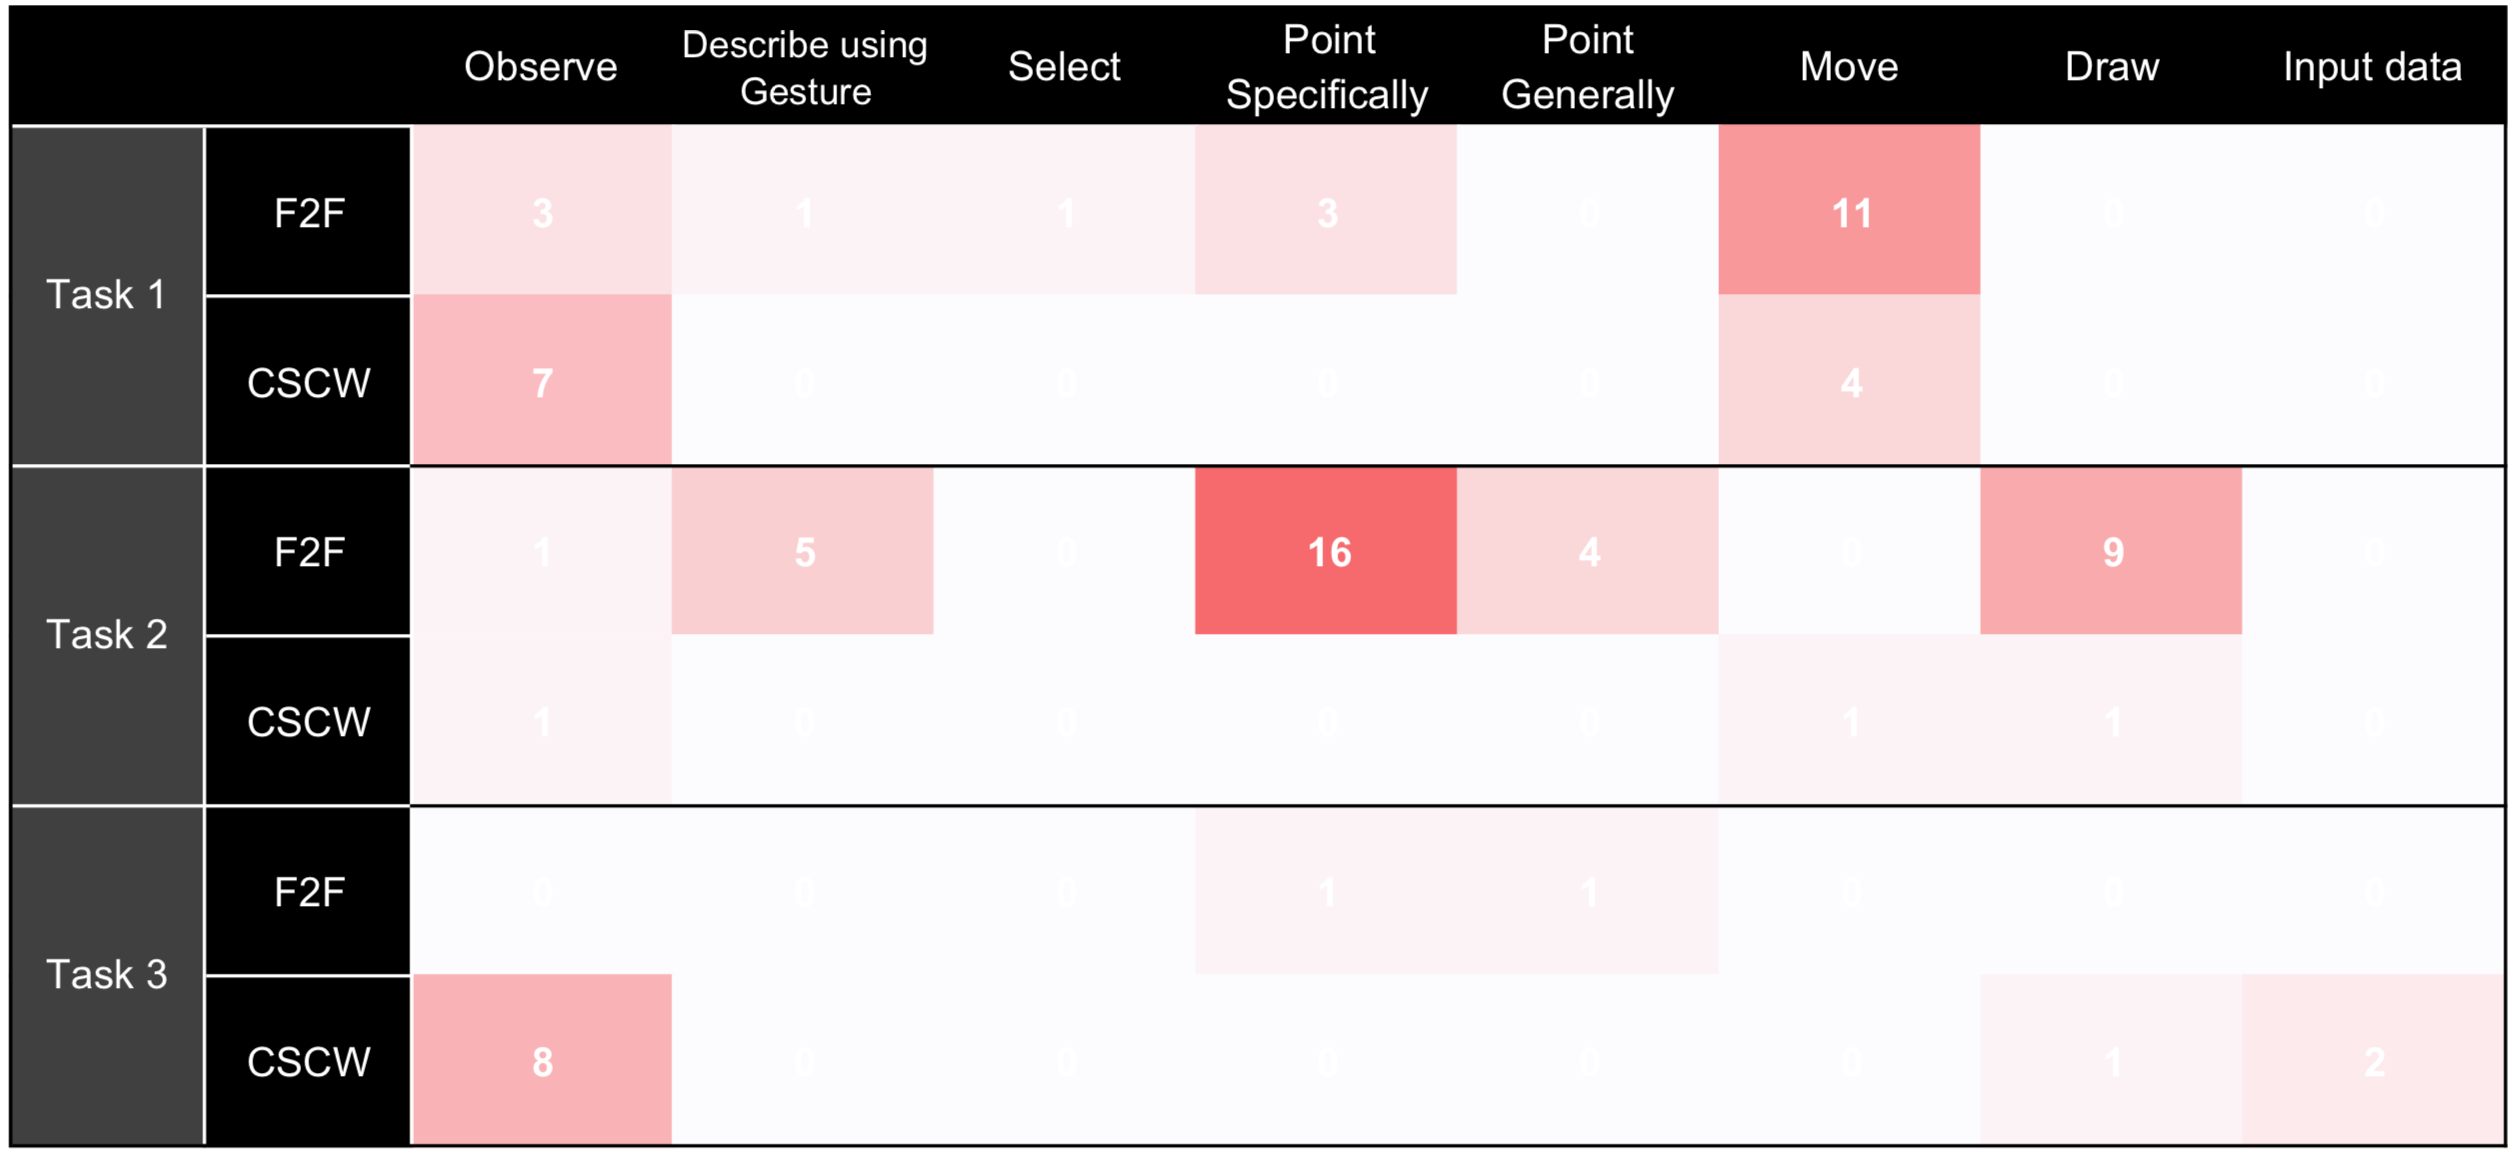
\includegraphics[width=\linewidth]{img/action_mode_a.png}
  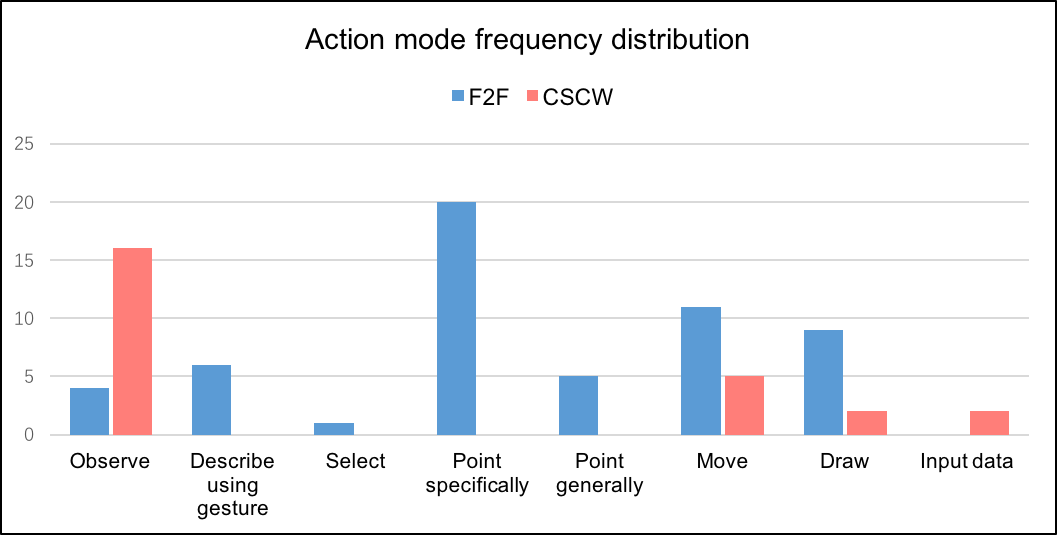
\includegraphics[width=\linewidth]{img/action_mode_b.png}
\endminipage\hfill
\minipage{0.27\textwidth}
  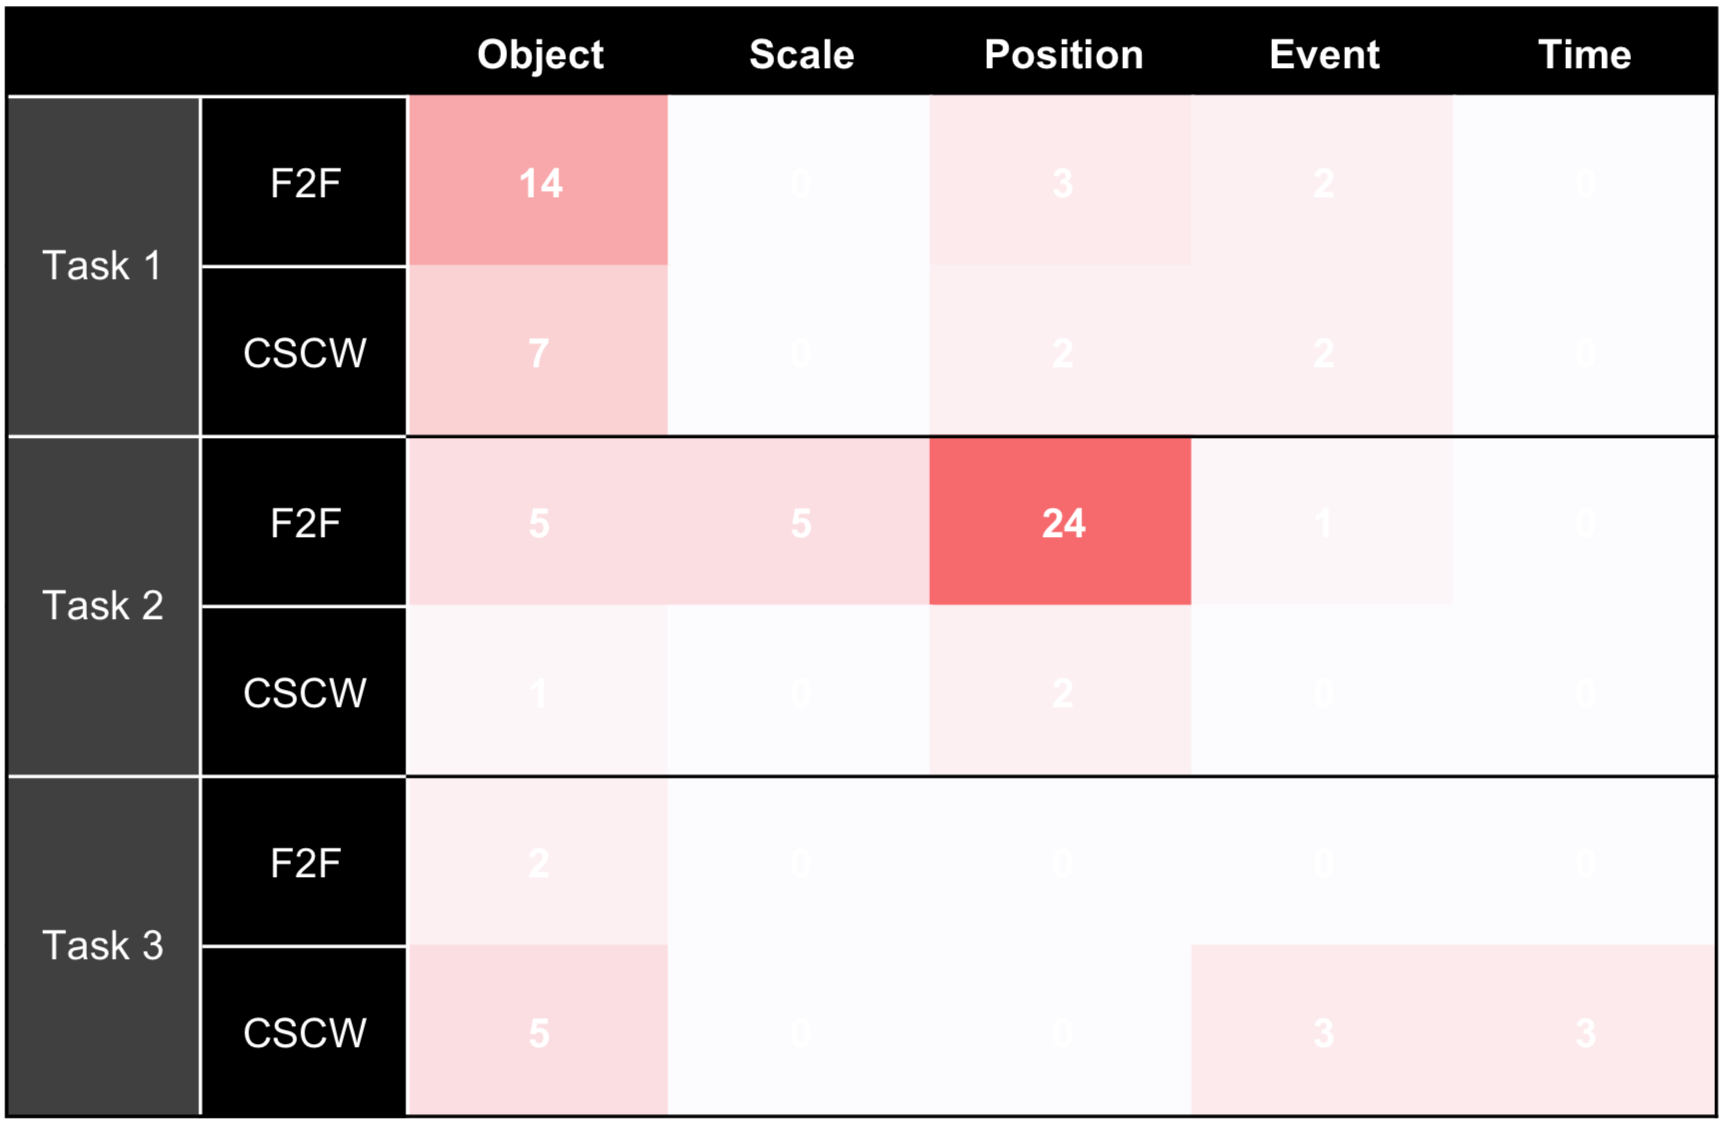
\includegraphics[width=\linewidth]{img/deixis_reference_a.png}
  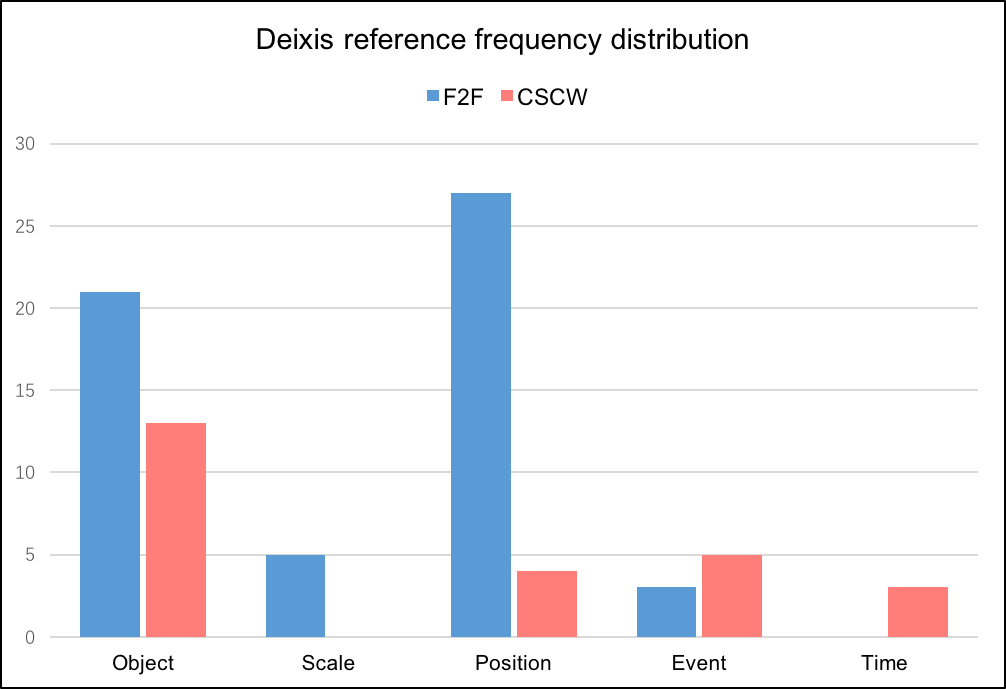
\includegraphics[width=\linewidth]{img/deixis_reference_b.png}
\endminipage\hfill
\minipage{0.265\textwidth}%
  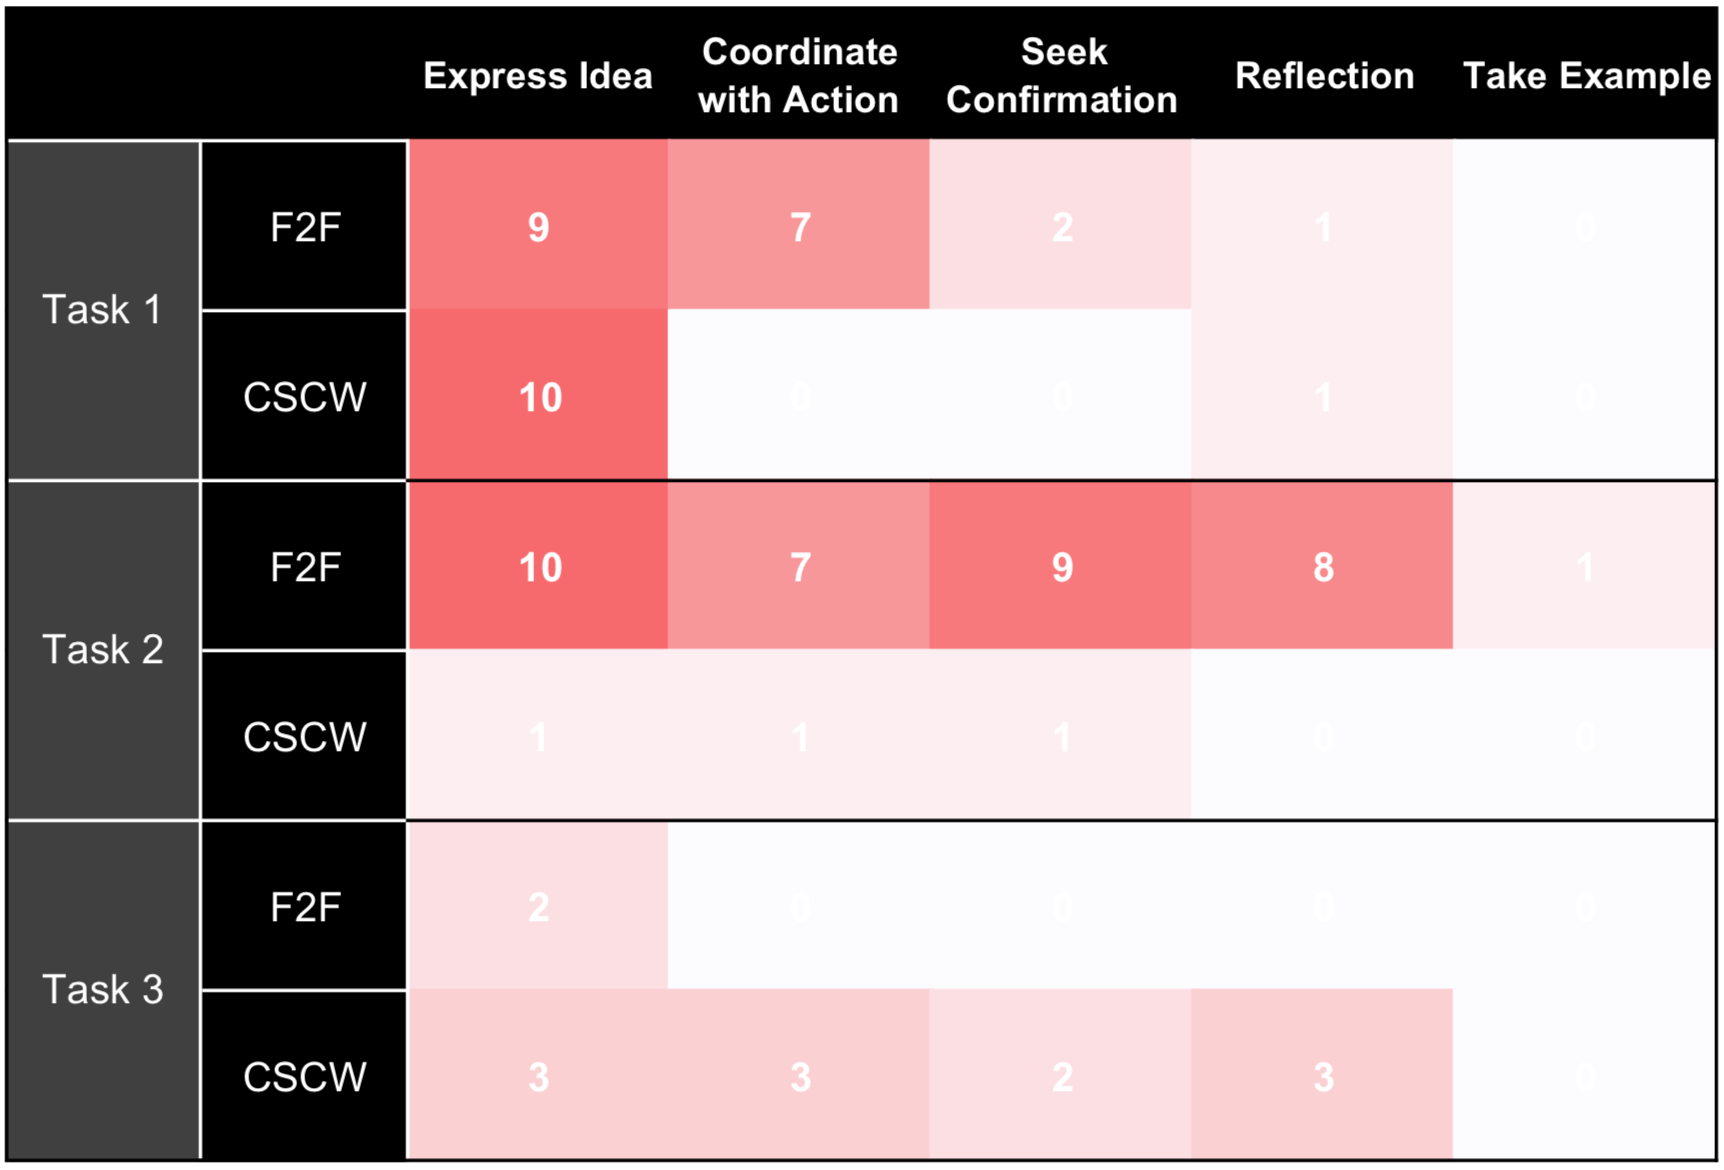
\includegraphics[width=\linewidth]{img/deixis_role_a.png}
  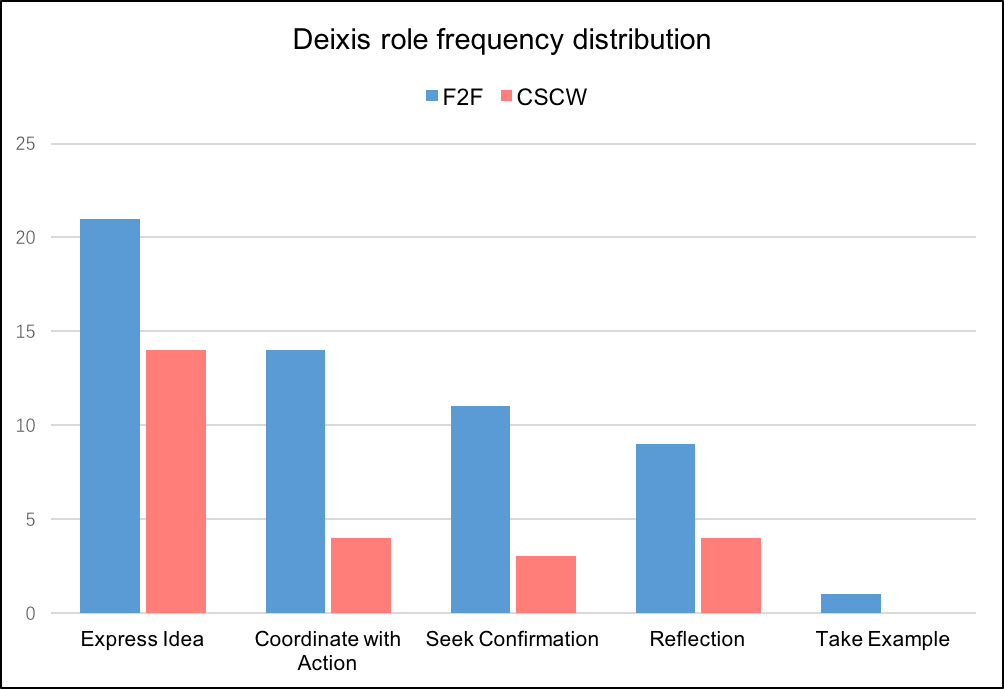
\includegraphics[width=\linewidth]{img/deixis_role_b.png}
\endminipage
\caption{From left to right: occurrence distribution of action mode, deixis reference and deixis role. Top row: occurrence distribution in each task, darker red corresponds to more significant occurrence. Bottom row: occurrence distribution across tasks}\label{fig:yumin}
\end{figure}

\begin{figure}
\minipage{0.47\textwidth}
  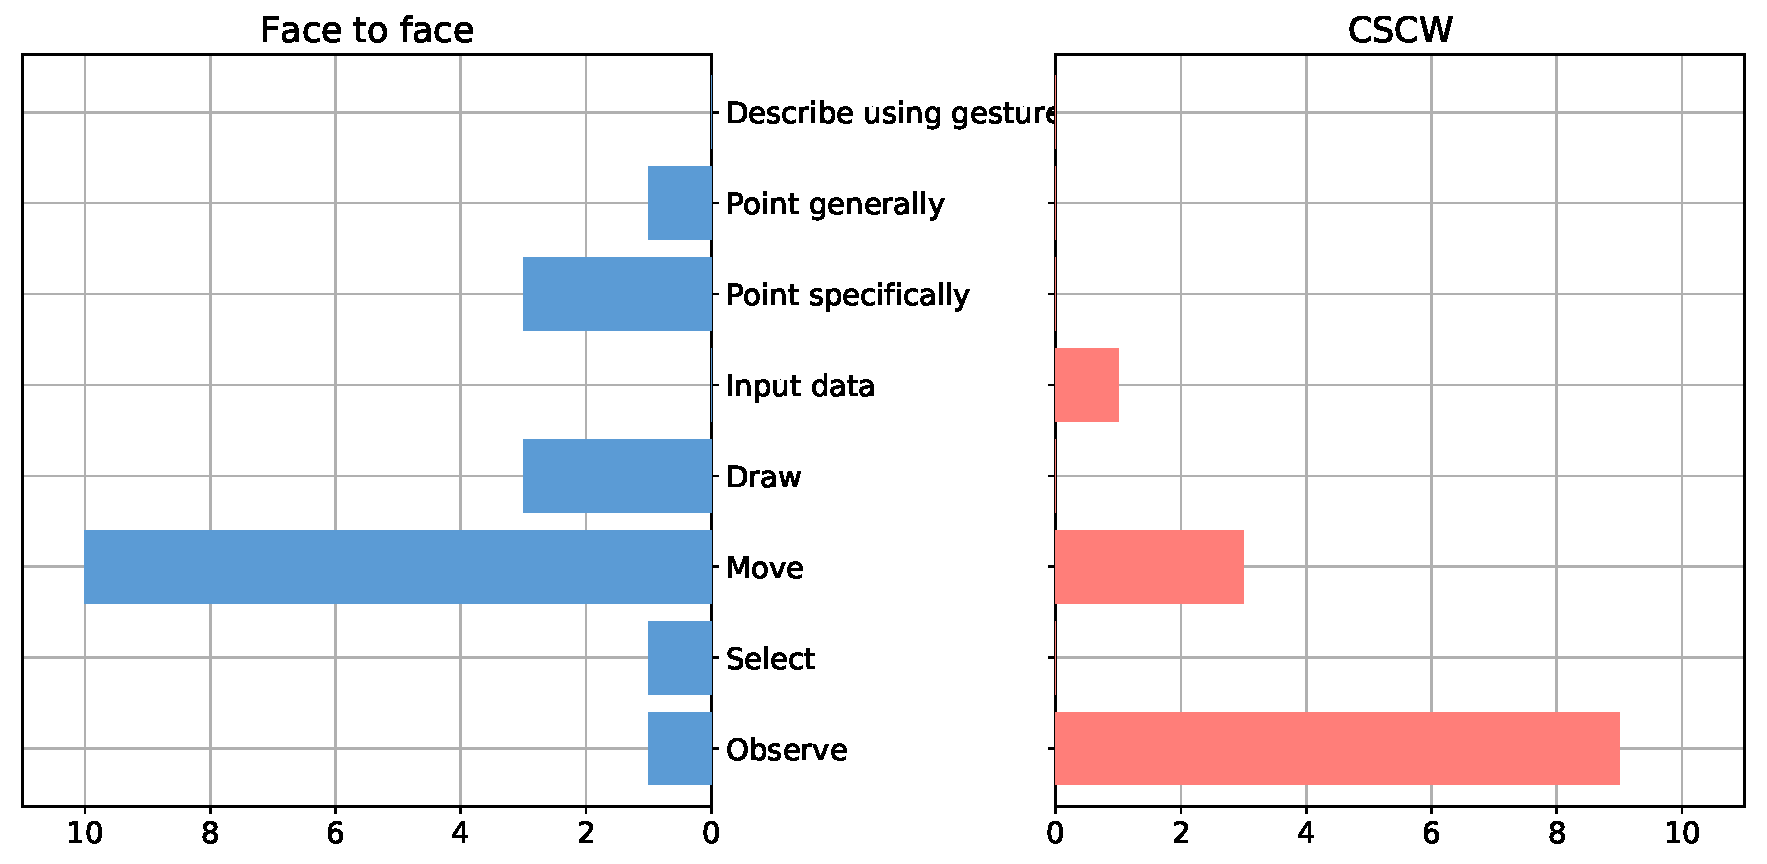
\includegraphics[width=\linewidth]{img/Object.pdf}
  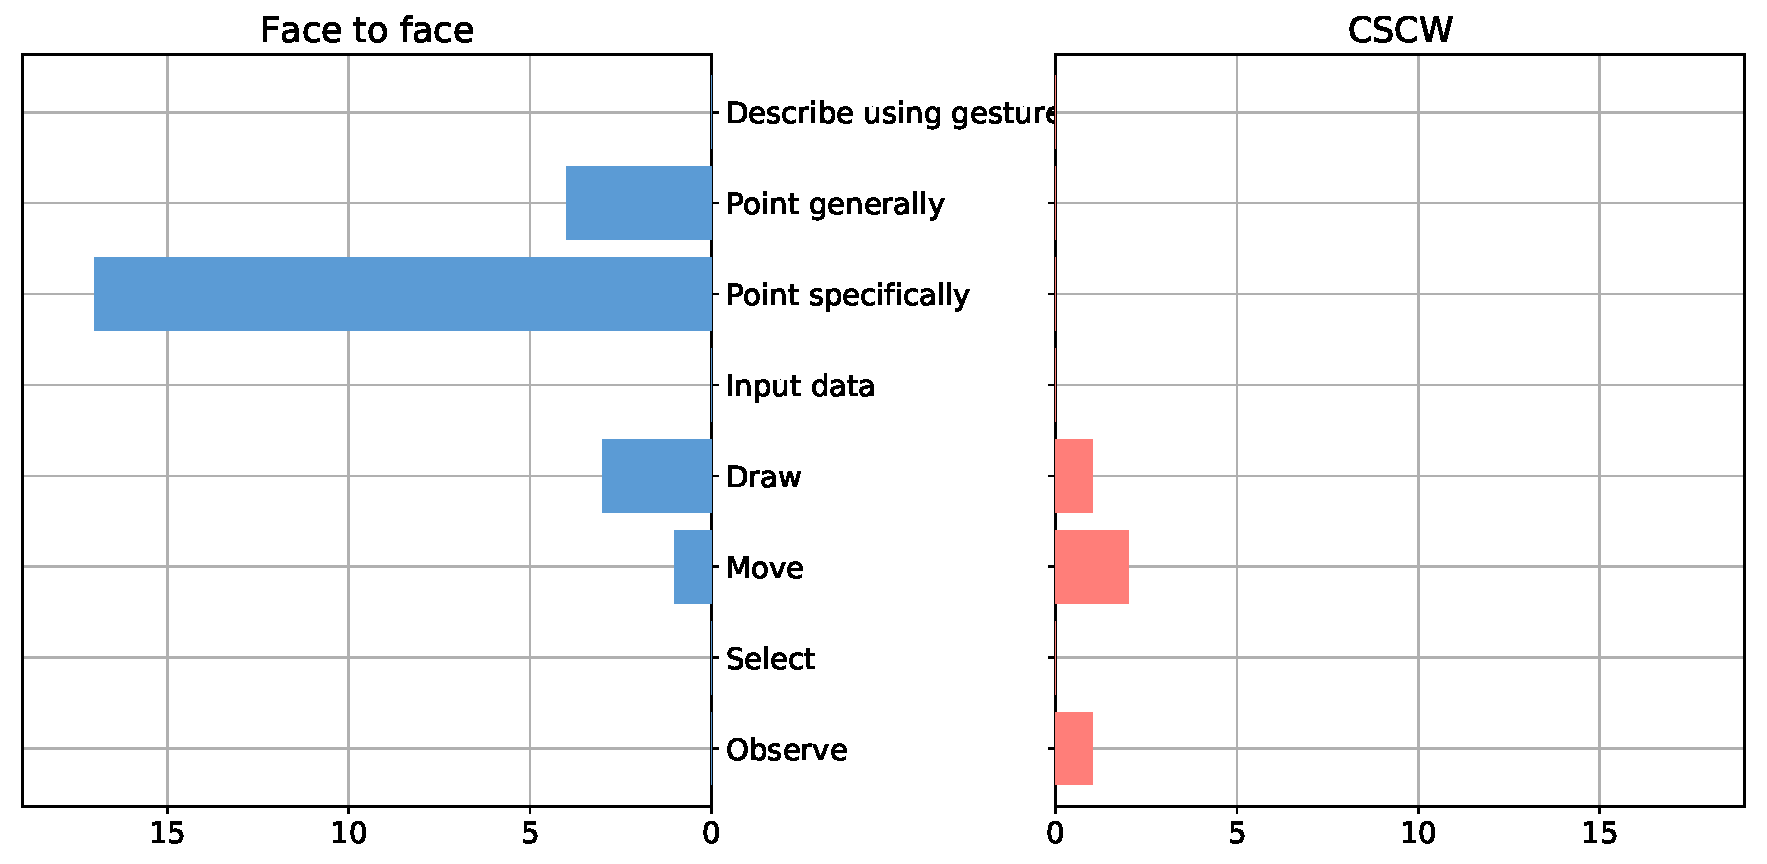
\includegraphics[width=\linewidth]{img/Position.pdf}
  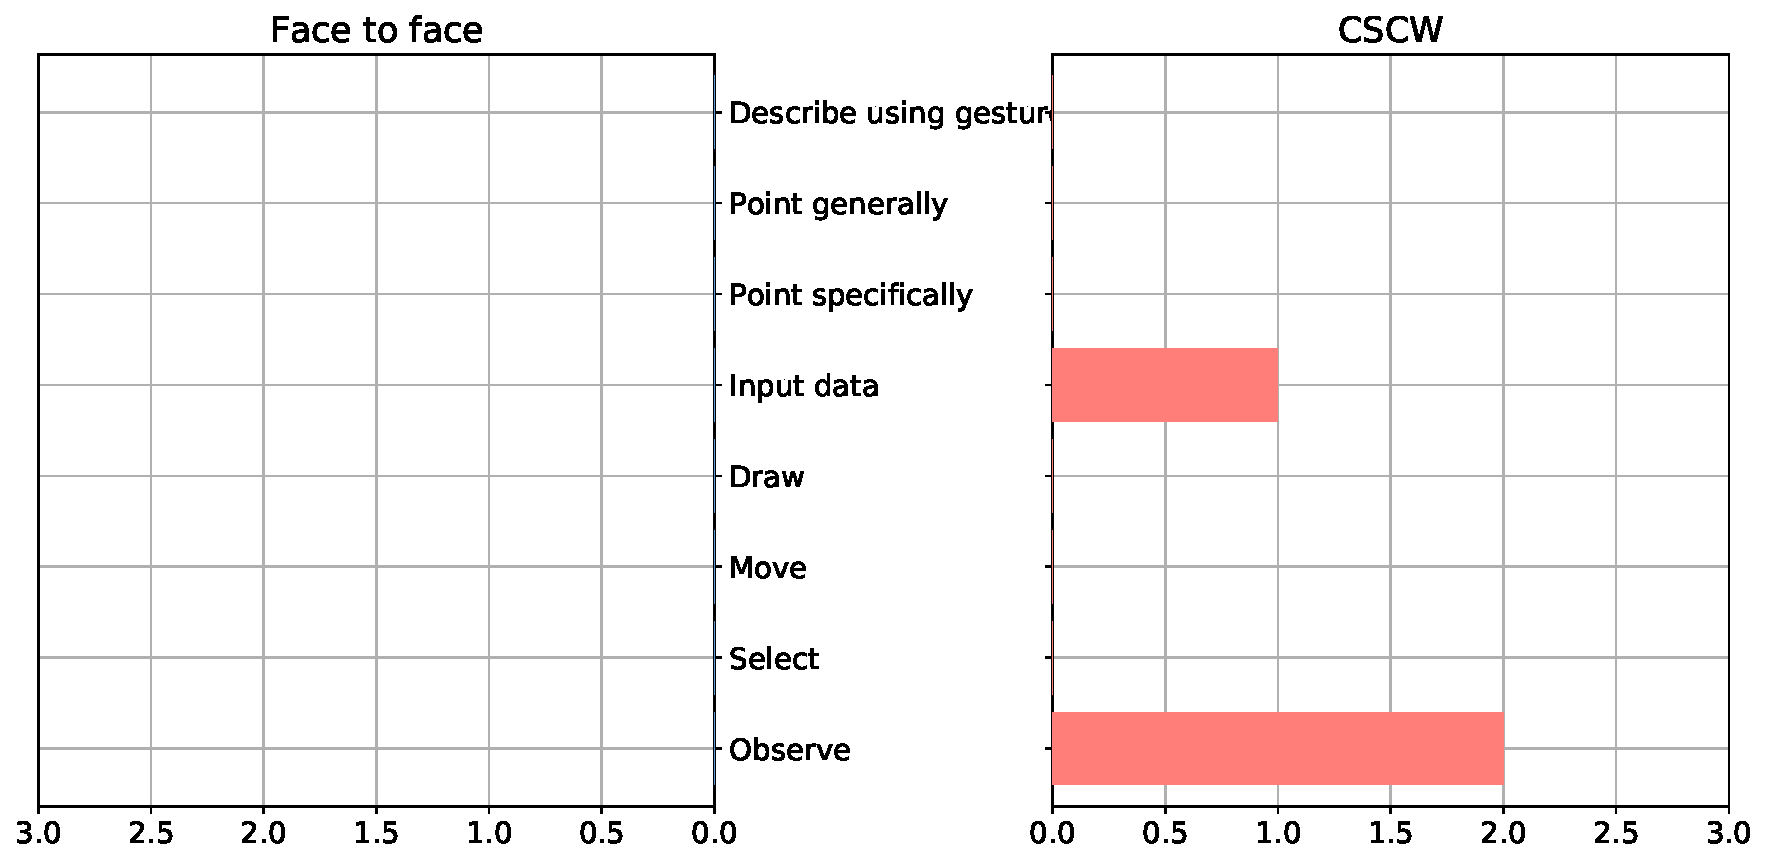
\includegraphics[width=\linewidth]{img/Time.pdf}
\endminipage\hfill
\minipage{0.47\textwidth}
  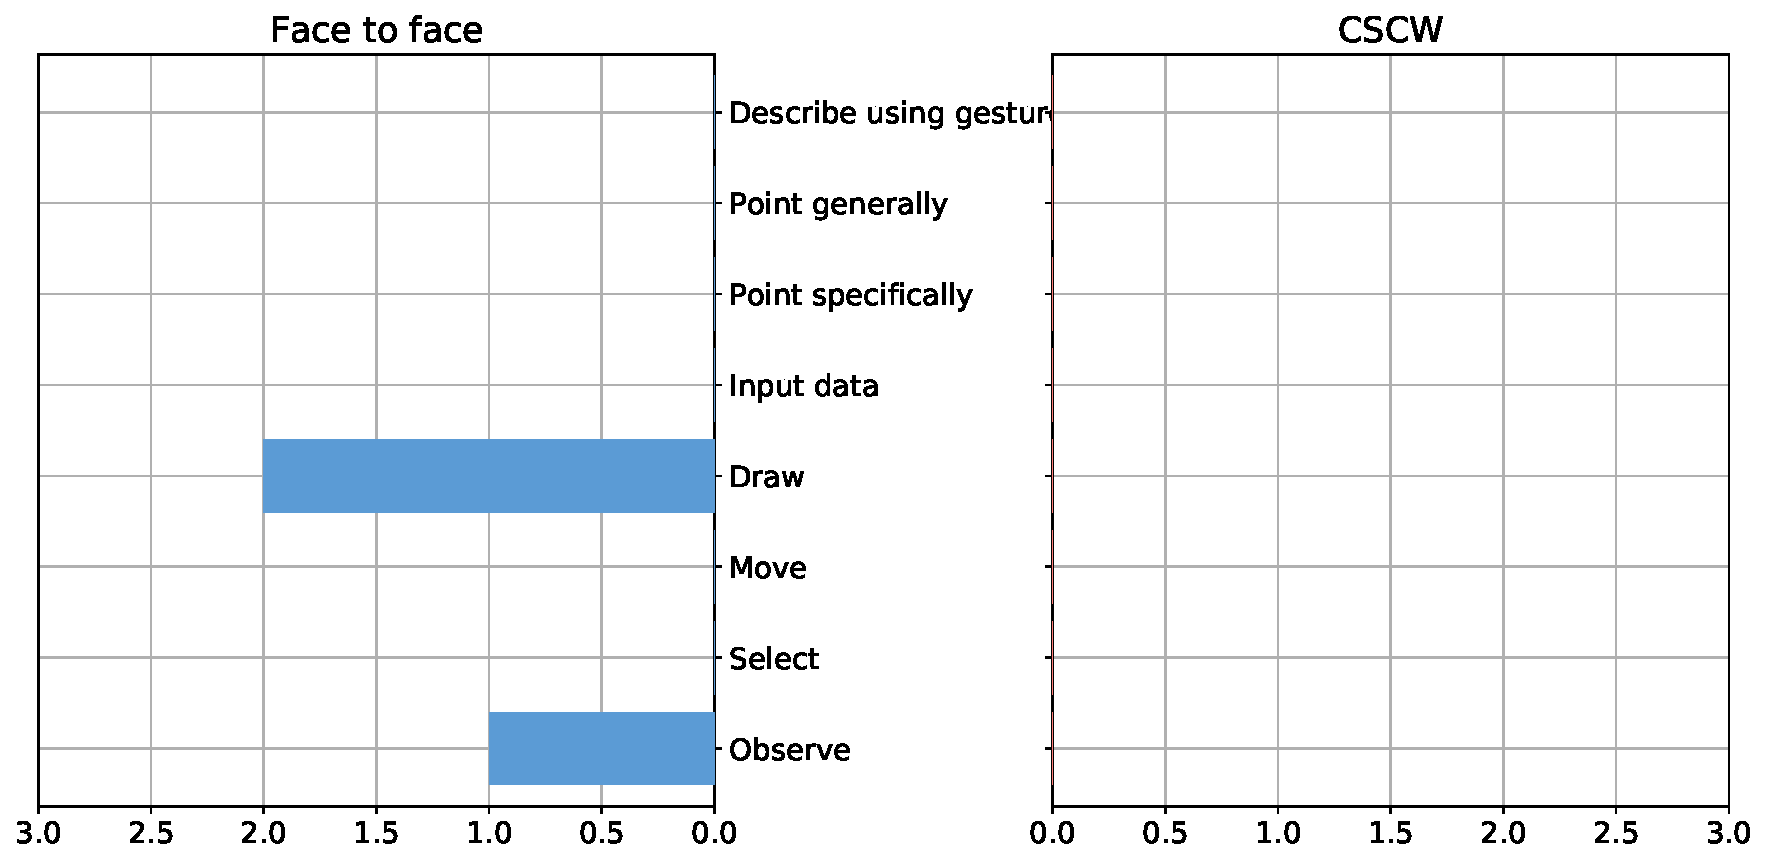
\includegraphics[width=\linewidth]{img/Scale.pdf}
  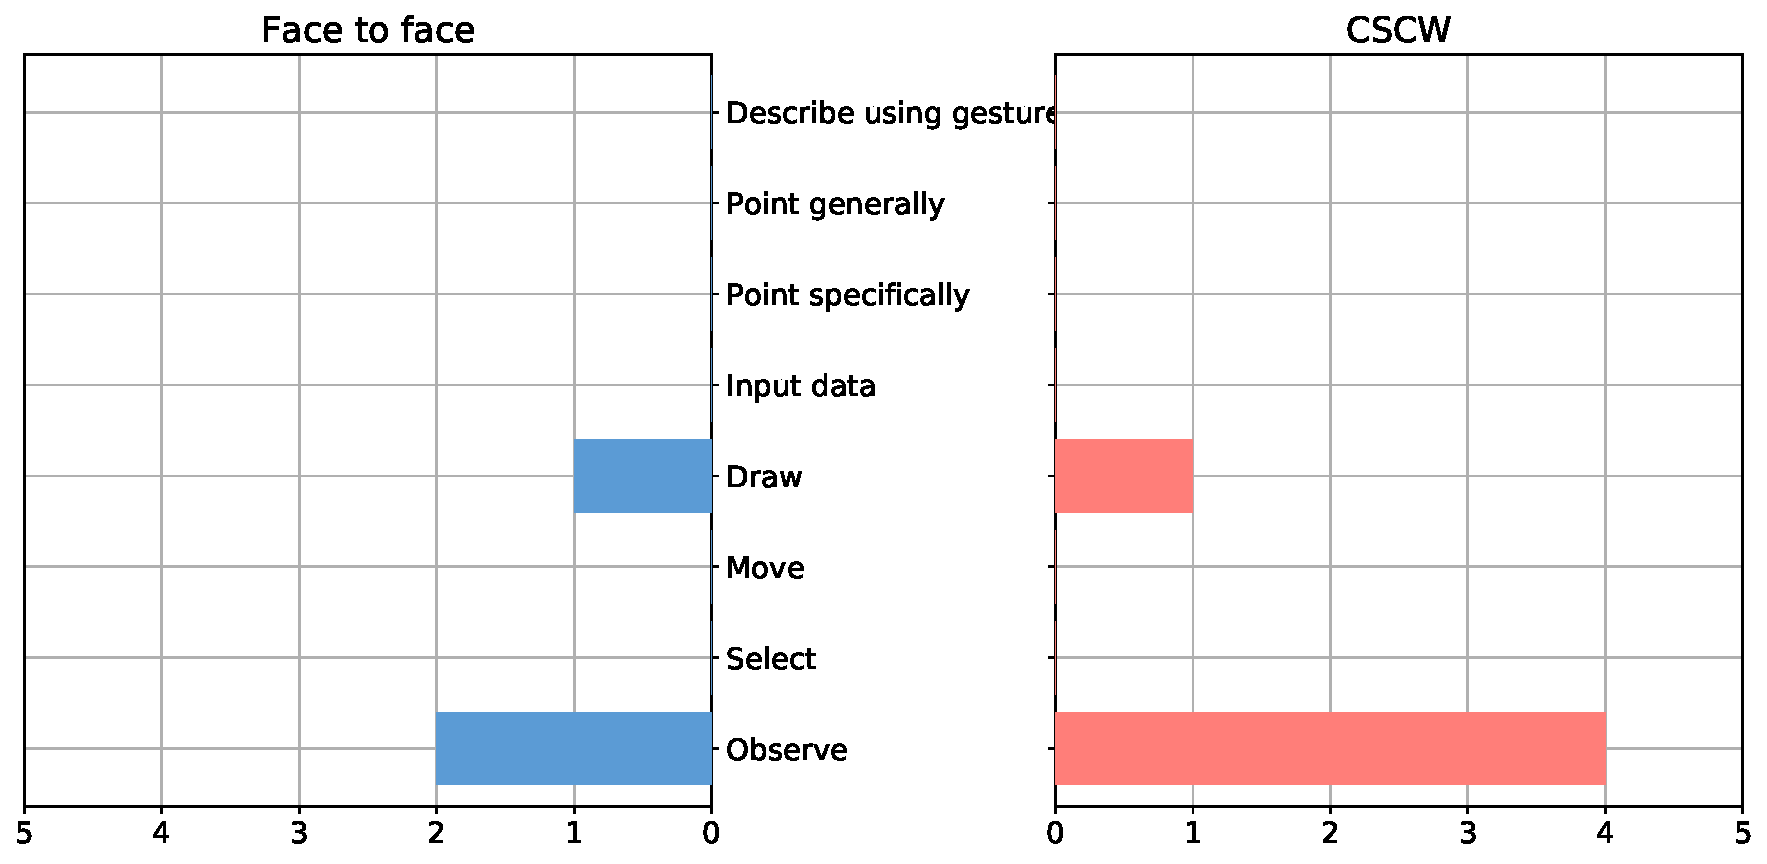
\includegraphics[width=\linewidth]{img/Event.pdf}
  \vspace{3.7cm}
\endminipage\hfill
\caption{Occurrence distribution of action modes for each deixis reference. Left column top-down: object, position, time. Right column top-down: scale, event}\label{fig:jiayao}
\end{figure}

We transcribed 81 deixis usage behaviour instances in total from our field experiment, with 56 instances from face-to-face condition, and 35 instances from CSCW condition. Then we analysed occurrence distribution of action mode, deixis reference and deixis role for each task and across tasks, see in figure \ref{fig:yumin}, and occurrence distribution of action mode in each deixis reference, see in figure \ref{fig:jiayao}, we compared those statistics in CSCW condition with face-to-face condition, and got the following analysis results.

\subsubsection{Observing played an important role in CSCW}
Deixis were used 37.5\% less in CSCW condition than face-to-face condition, with 42.1\% less in task 1 (puzzle), and 91.4\% less in task 2 (room layout design), whilst in task 3 (storyboard design) deixis were used more often in CSCW due to more observing as deixis behaviours. As task 3 was strongly dependent on task 2, designing a storyboard based on room layout, we assume two collaborators got familiar with the collaborations during task 2, so that they didn't need too much deixis to communicate and coordinate, and instead they can collaborate using certain tacit agreement during task 3. From the left chart in figure \ref{fig:yumin} we also found observing action mode pop out. It was the most frequently used action mode in CSCW condition across all tasks, especially in task 3. We went back to transcribed action and saying in the video, found that when collaborators were operating on the same object in CSCW condition, they tended to observe to understand intention and action of collaborator, to avoid conflicts and coordinate collaboration, like saying ``is it finished?" ``you did it very clearly".

\subsubsection{Position, object and scale were the most needed deixis reference}

From the middle chart in figure \ref{fig:yumin} we can see position, object and scale were the most frequently happened deixis references both in face-to-face and CSCW conditions. In task 1, when collaborators were operating on predefined puzzle pieces, they more frequently used deixis referring to objects. In task 2, when collaborators were drawing room layout from scratch, their started to express scales and positions by deixis, especially to express positions, which took up 68.6\% among all five deixis references under face-to-face condition. By contrast, collaborators used deixis refer to positions much less in CSCW conditions, as there were 24 such instances in face-to-face condition, but only 2 such instances in CSCW condition. It was a significant finding that the most used deixis behaviour in face-to-face condition had pretty limited instances in CSCW condition.

\subsubsection{No pointing and less moving were used in CSCW}
As shown in the left chart in figure \ref{fig:yumin}, pointing specifically and generally were frequently appeared action modes in face-to-face condition, taking up 20.8\% among all eight action modes, while 80\% of the pointing happened in task 2. However, there were no pointing used at all in CSCW condition. It could because of the CSCW platform we used - RealTime Board app on two iPads, since pointing to an element on its drawing interface on one end would not result to any visible indication on another end, namely collaborators can not use pointing to convey information in CSCW condition with our experimented platform. In terms of pointing per se, 80\% of the pointing are pointing specifically, like ``let's place the door in this corner", rather than pointing generally, like ``can the bed orient here'' with pointing to one side of drawing paper. From the left top and middle charts in figure \ref{fig:jiayao}, we found that pointing were used to refer to object and position, especially pointing specifically to express position, account for 84\% of all the pointing. Similarly, in task 1, collaborators often used movings to refer to objects in face-to-face condition, which was a further enhancement to situate attention compared to pointing, while in CSCW condition moving were 63.6\% less then the ones in face-to-face condition.

\subsubsection{Deixis referring to event and time were needed across face-to-face and CSCW}

From the middle chart in figure \ref{fig:yumin} we can see that while overall deixis usage were shrinking in CSCW condition, deixis referring to event and time remained certain occurrence, like ``can I type now? (input data)'',``just do it like planned''. Though event and time as deixis references were as frequent as position, object, and scale, we still can derived that deixis references to event and time are universally needed across collaborations, wherever face-to-face collaboration or CSCW. Furthermore, as shown in the right middle and left bottom charts in figure \ref{fig:jiayao}, collaborators observed more when using deixis refer to event and time in CSCW condition, we considered it resulted from lack of contextual information that collaborators have to infered the context they needed from observing the CSCW drawing interface.

\subsubsection{Expressing an idea was the most needed deixis conceptual purpose}

According to the right chart in figure \ref{fig:yumin}, deixis role as expressing an idea was always the most frequently happened across all tasks in both face-to-face and CSCW condition. From our recorded actions and sayings from the video, collaborators expressed themselves by ``this piece could be next to it'' (in task 1),``the desk can be here, the keyboard can be there'' (in task 2),``I can type here'' (in task 3). In addition, we also found that for task 1 in CSCW condition, namely collaborators were operating on predefined puzzle pieces, they still kept almost the same frequency to express themselves as in face-to-face condition, whilst for task 2 in CSCW condition, when collaborators were drawing room layout, they used much less deixis to express an idea along with the overall shrinking of deixis usage.

\section{Discussion}
\label{sec:discussion}
On top of those key findings from the field experiment, we identified the most significant design improvement possibilities. As overall deixis usage were lessen in CSCW condition, and collaborators paid more observing across tasks, it suggested collaborators turned active deixis expression in face-to-face condition to passive indication observation in CSCW condition. One step further, collaborators still do have needs to perceive contextual information originally carried by deixis in face-to-face condition, but they were limited to express and perceive deixis in CSCW condition.

In terms of expression purpose, since collaborators most frequently used deixis to express position, object and scale across face-to-face and CSCW conditions, and it is noteworthy that position, the most used deixis reference in face-to-face condition, whilst got decreased its usage the most as in CSCW condition, we should prioritize in collaborative drawing groupware interaction design, to facilitate the expressions of position, object and scale, especially position.

Furthermore, as for how collaborators use deixis to communicate, considering we chose RealTime Board app on iPads as our CSCW experiment platform, there were no pointing and less moving performed by collaborators in CSCW condition, while collaborators used pointing to express position and object mostly, especially position, and used moving to refer to an object. From another angle, when collaborators were referring to a position, they used pointing mostly, when they refer to an object, the most frequent actions were moving and pointing. From this point we could think about how to design interactions in groupware to enable the expressions by those action modes.

Then we specify our design problems as ``how to support the deixis usage to refer to positions, scales and objects in CSCW”. The challenges come from multiple interpretations on single hand gesture. For example, a touchpoint received from the groupware backend, could be interpreted as drawing, moving and even selecting, and each interpretation could yield different function and feedback from the groupware, like drawing a curvature, moving an object, and highlight an object. We divided these functions into two categories, gesture function 1 group supports drawing operations, and gesture function 2 group enables the deixis usages. Admittedly, there is ambiguous interpretations on hand gestures, as shown in the table \ref{tab:tableconflict}, and there are some techniques to solve this issue: using different devices (such as drawing pen and gesture pen), selecting different modes (such as gesture mode and drawing mode), or tense detection (such as holding down a button on the pen to indicate a gesture) \cite{buxton1986chunking}. Additionally, in project Tivoli \cite{pedersen1993tivoli}, a double tap on the pen was used, as the postfix indicator. In our design sketches, we used a technique similar to the selection of different modes, but with new interactions.

\begin{table}
  \centering
  \begin{tabular}{l l l}
    % \toprule
    {\small\textit{Hand Gesture}}
    & {\small \textit{Gesture Function 1 (drawing)}}
    & {\small \textit{Gesture Function 2 (communication)}} \\
    \midrule
    Tap screen & Select & Indicate a position or an object \\ 
    Slide & Move & Indicate direction \\ 
    Pinch & Zoom in/Zoom out & Indicate a scale \\
    Draw & Draw & Gesticulating \\ 
    % \bottomrule
  \end{tabular}
  \caption{The same hand gestures can express and enable different operations}~\label{tab:tableconflict}
\end{table}

\subsection{Groupware interaction design}
\label{sec:design}
Here we propose our final interaction design for collaborative drawing groupware. On the drawing canvas of a touch interface, we added a second layer, a transparent indication layer. The idea was using two layers to contain two sets of gesture functions: Drawing function and Communicating function. We designed a button to toggle between two layers. The design sketch is illustrated in figure \ref{fig:design1_a}. The user can use the same set of hand gestures to enable two sets of functions, one set per layer, which is further illustrated in the table \ref{tab:design1_b}. The actions performed on the indication layer would not affect the final drawing on drawing canvas. 

\begin{figure}
\minipage{0.49\textwidth}
  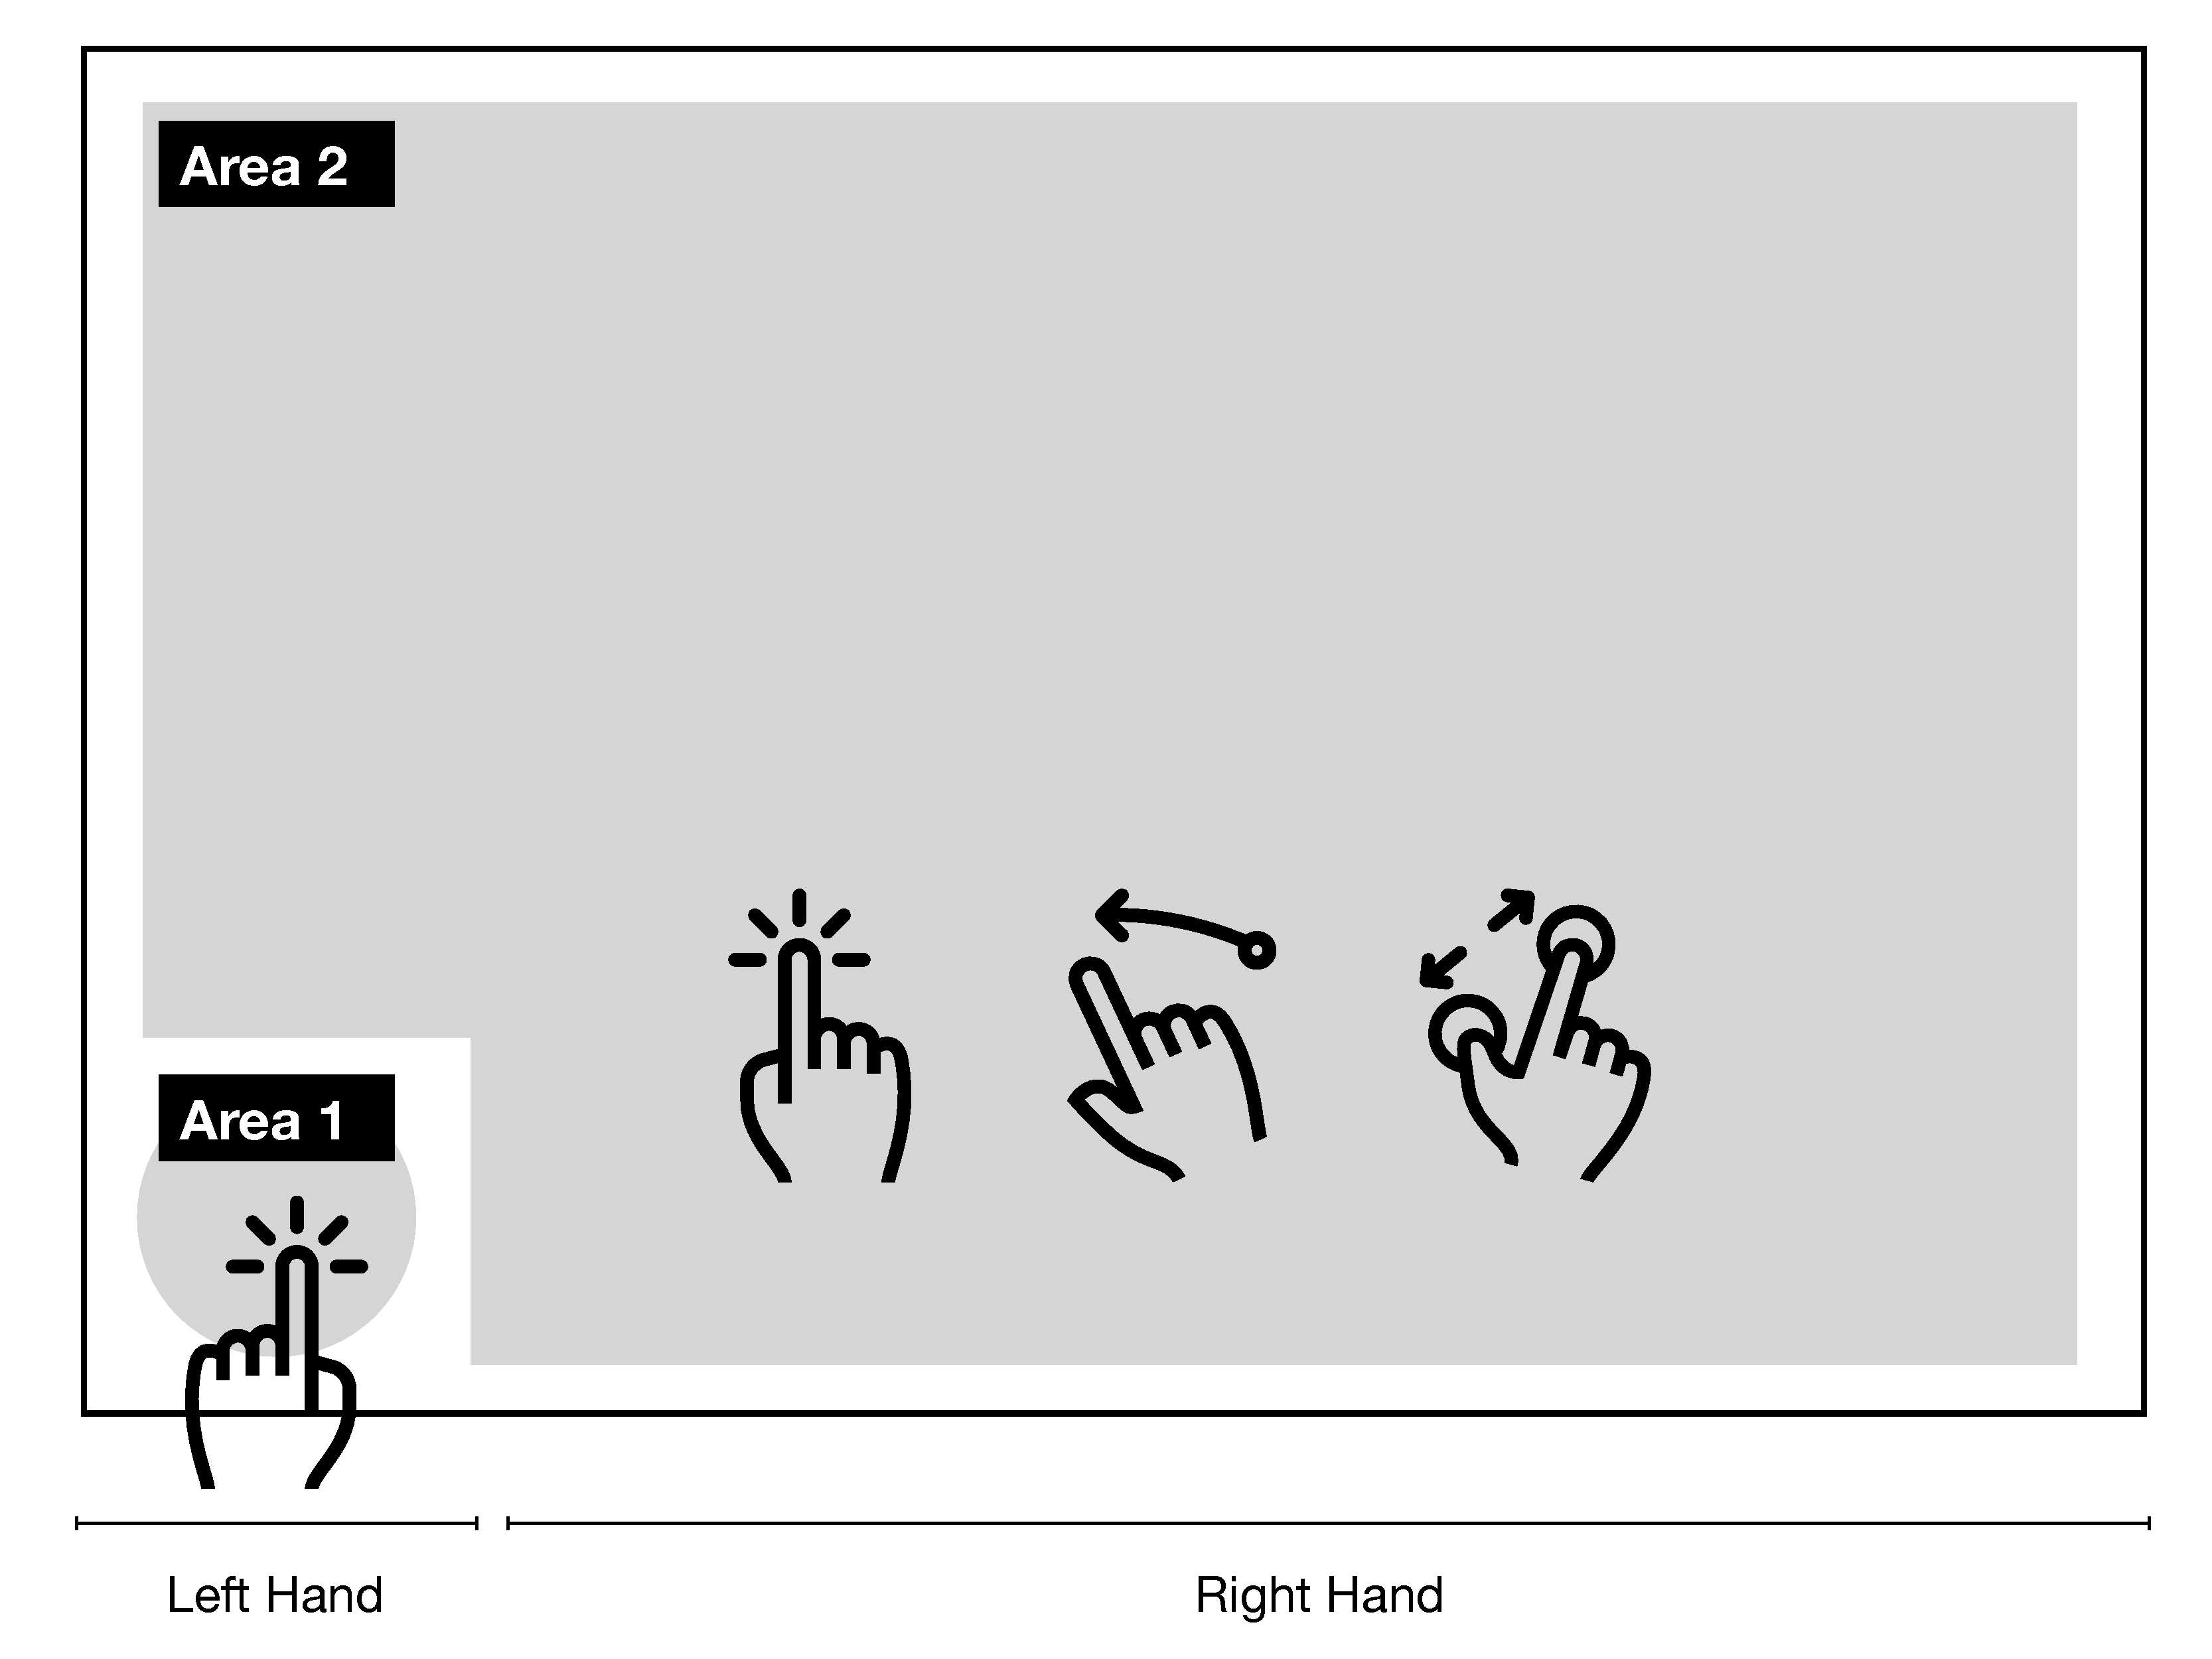
\includegraphics[width=\linewidth]{img/design1_structure.pdf}
\endminipage\hfill
\minipage{0.49\textwidth}
  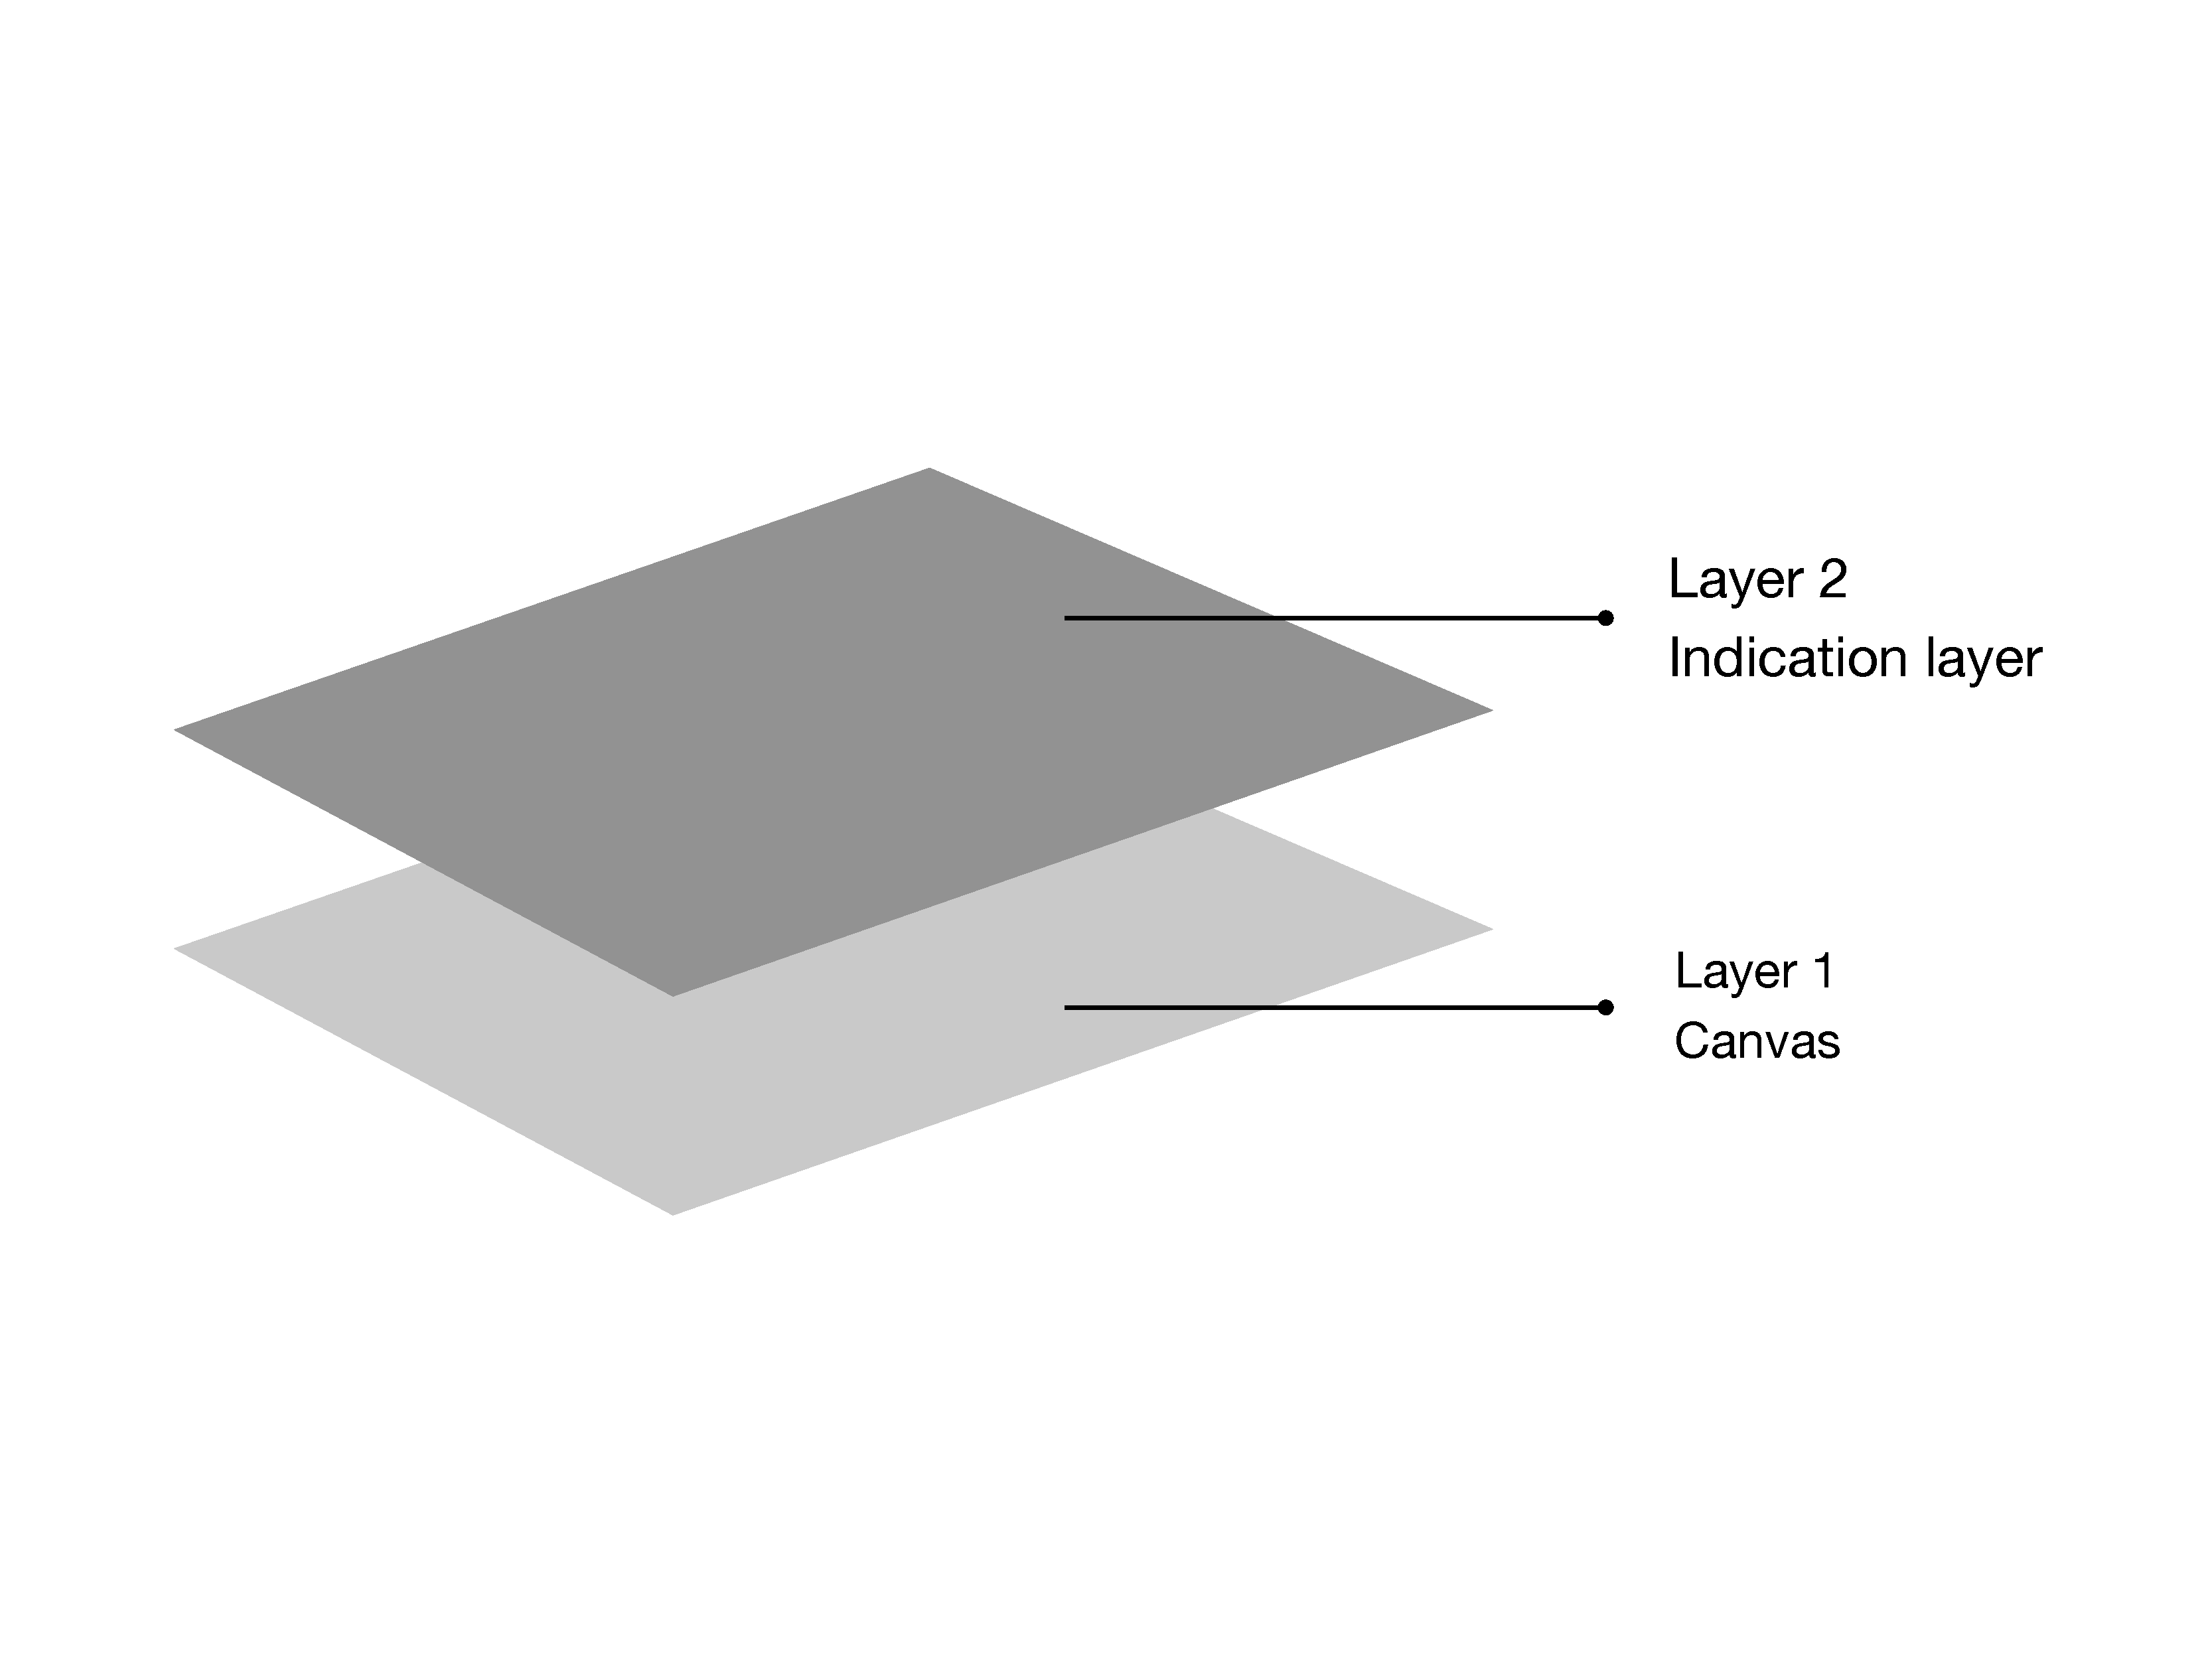
\includegraphics[width=\linewidth]{img/design1_layer.pdf}
\endminipage\hfill
\caption{Interaction design structure}\label{fig:design1_a}
\end{figure}

\begin{table}
  \centering
  \begin{tabular}{l l l l}
    % \toprule
    {\small\textit{Left hand: Area 1}}
    & {\small \textit{Right hand: Area 2}}
    & {\small \textit{ }} 
    & {\small \textit{ }} \\
    \midrule
    Button status & Gesture & Layer 1 & Layer 2 \\
     \midrule
       Unpressed & Tap/Pressed & Select & Invalid \\
       & Slide & Move & Invalid \\
       & Pinch & Zoom in/Zoom out & Invalid \\
       & Draw & Draw & Invalid \\
     \midrule
    Button status & Gesture & Layer 1 & Layer 2 \\
     \midrule
     Pressed  & Tap/Pressed & Invalid & Indicate a place or an object \\
       & Slide & Invalid & Indicate a direction \\
       & Pinch & Invalid & Indicate a scale \\
       & Draw & Invalid & Sketch or scope in the air \\
    % \bottomrule
  \end{tabular}
  \caption{Interaction description}~\label{tab:design1_b}
\end{table}

By this interaction design, we utilised the advantages from two-handed operation, allowing the users to perform their drawings as well as express deixis within the drawing interface.

To evaluate our interaction design concept, once again, we invited the two test subjects who participated in our field experiment, because they have gotten familiar with the deixis usage problems encountered in CSCW and would have deeper feedbacks on our improvement scheme. Moreover, we designed two tasks in this evaluation session, as shown in appendix \ref{appdx:evaluationtask}. In the first task we have test subjects use deixis to express their own ideas, while in the second task we have test subjects ask their collaborators to do something. This two tasks are related to previous tasks in the field experiment: room layout design and puzzle. In addition, considering our prototype is a design concept, we used cognitive walkthrough method \cite{polson1992cognitive} and think aloud testing \cite{boren2000thinking} to conduct our evaluation test.

The test began with a description of our design concept. We introduced the design goal, user interface, and main interaction of our prototype. After understanding how to use this interface, we instructed them with cognitive walkthrough method, encouraged them to think aloud what they thought and how they felt during performing the tasks. Finally the test subjects were asked to give some improvement feedbacks freely.

We recorded the evaluation from observations on performing tasks, thinking aloud utterance and subjective feedback after the whole test. Surprisingly, the two test subjects spoke high of this design concept and said "that is a easy way to solve this problem. Easy to learn, and easy to interact with." Just as what we observed in the test, they knew how to perform each task efficiently and acted appropriately. However, according to the feedback from one of the test subjects, it was troublesome to switch layer mode too often. Instead, using an indicator to show which layer is currently enabled and giving an intelligent undo or eraser function could help. Furthermore, they were concerned that they may prone to errors if they have worked with it for a long time.    

\subsection{Limitations and future work}
\label{sec:limitations}
We analysed that the limitations of our research reside in three aspects. In our field experiment, though we used two different task-sets for face-to-face and CSCW condition respectively, this two task-sets still have certain similarity. Test subjects might get familiar with the tasks from the practices in face-to-face session, therefore they spent less efforts in communication and coordination and had less deixis usage in CSCW session. In addition, we designed the third tasks were having test subjects design the storyboard in the space of six rectangles, while we observed in the field experiment, they divided tasks and drew three rectangles each person, thus it discounted the interactive collaboration and active deixis usage. As for the RealTime Board app on iPads as CSCW experiment platform, both test subjects used this app for the first time, thus they might be cautious to perform actions within the app including pointing, selecting, moving and etc. In addition, drawing with physical paper and pen, with fingertips on touchscreen and with digital pen on touchscreen have inherent differences. We experimented the drawing with fingertips on touch screen in CSCW session, the cost to toggle moving and drawing is higher than the one when drawing with physical pen and paper, since the test subjects have to toggle between ``selection'' and ``drawing'' from the app toolbar. Last but not least, considered the workload and the focus of this research, we aimed to go through the research pipeline properly instead of collecting data per se, we only invited two test subjects. In a fully treated research, the researchers could have more test subjects and more data.

In terms of our research question formulation and data analysis, we didn't investigate the deixis usage during the collaboration involving multiple people, and only anlaysed the occurrence distribution using our data encoding framework. As mentioned by Tang et al. \cite{tang1991findings}, collaborators often combine their activities fluently in the drawing space. From this point, we didn't research its effect and significance of each action mode in those combinations.

The design sketch left lot of room for improvement as well. We adopted the concept that determine gesture interpretations between communication and drawing by containing action modes in two layers. However, this method requires the user to switch mode frequently and quickly under intensive collaborations. If communicating and drawing are interwoven, it would be demanding for the users to switch the layers and have them prone to errors. 

As for the future work, we encourage the research on deixis usage in the collaboration involving multiple people, and model intentions and status of collaborators from their actions and sayings using bigger set of data collected from hardware sensors and data mining, machine learning methods.

\bibliography{II2202-report}
%%\bibliographystyle{IEEEtran}
\bibliographystyle{myIEEEtran}
\appendix
\section{Field experiment user tasks}
\label{appdx:user tasks}

We designed two task-sets for face-to-face collaboration and CSCW setups respectively, each task-set consists of three tasks, corresponding tasks in two setups have equivalent content but with different descriptions and requirements. Detailed instructions given to test subjects are the follows.\\

Task 1, \textit{puzzle}.

Instructions were the same for both face-to-face collaboration and CSCW: In this task, please collaborate with your partner, finish this 9-piece puzzle in five minutes. 

The two puzzle images are shown in figure \ref{fig:field_task1}. \\

\begin{figure}[h!]
\centering
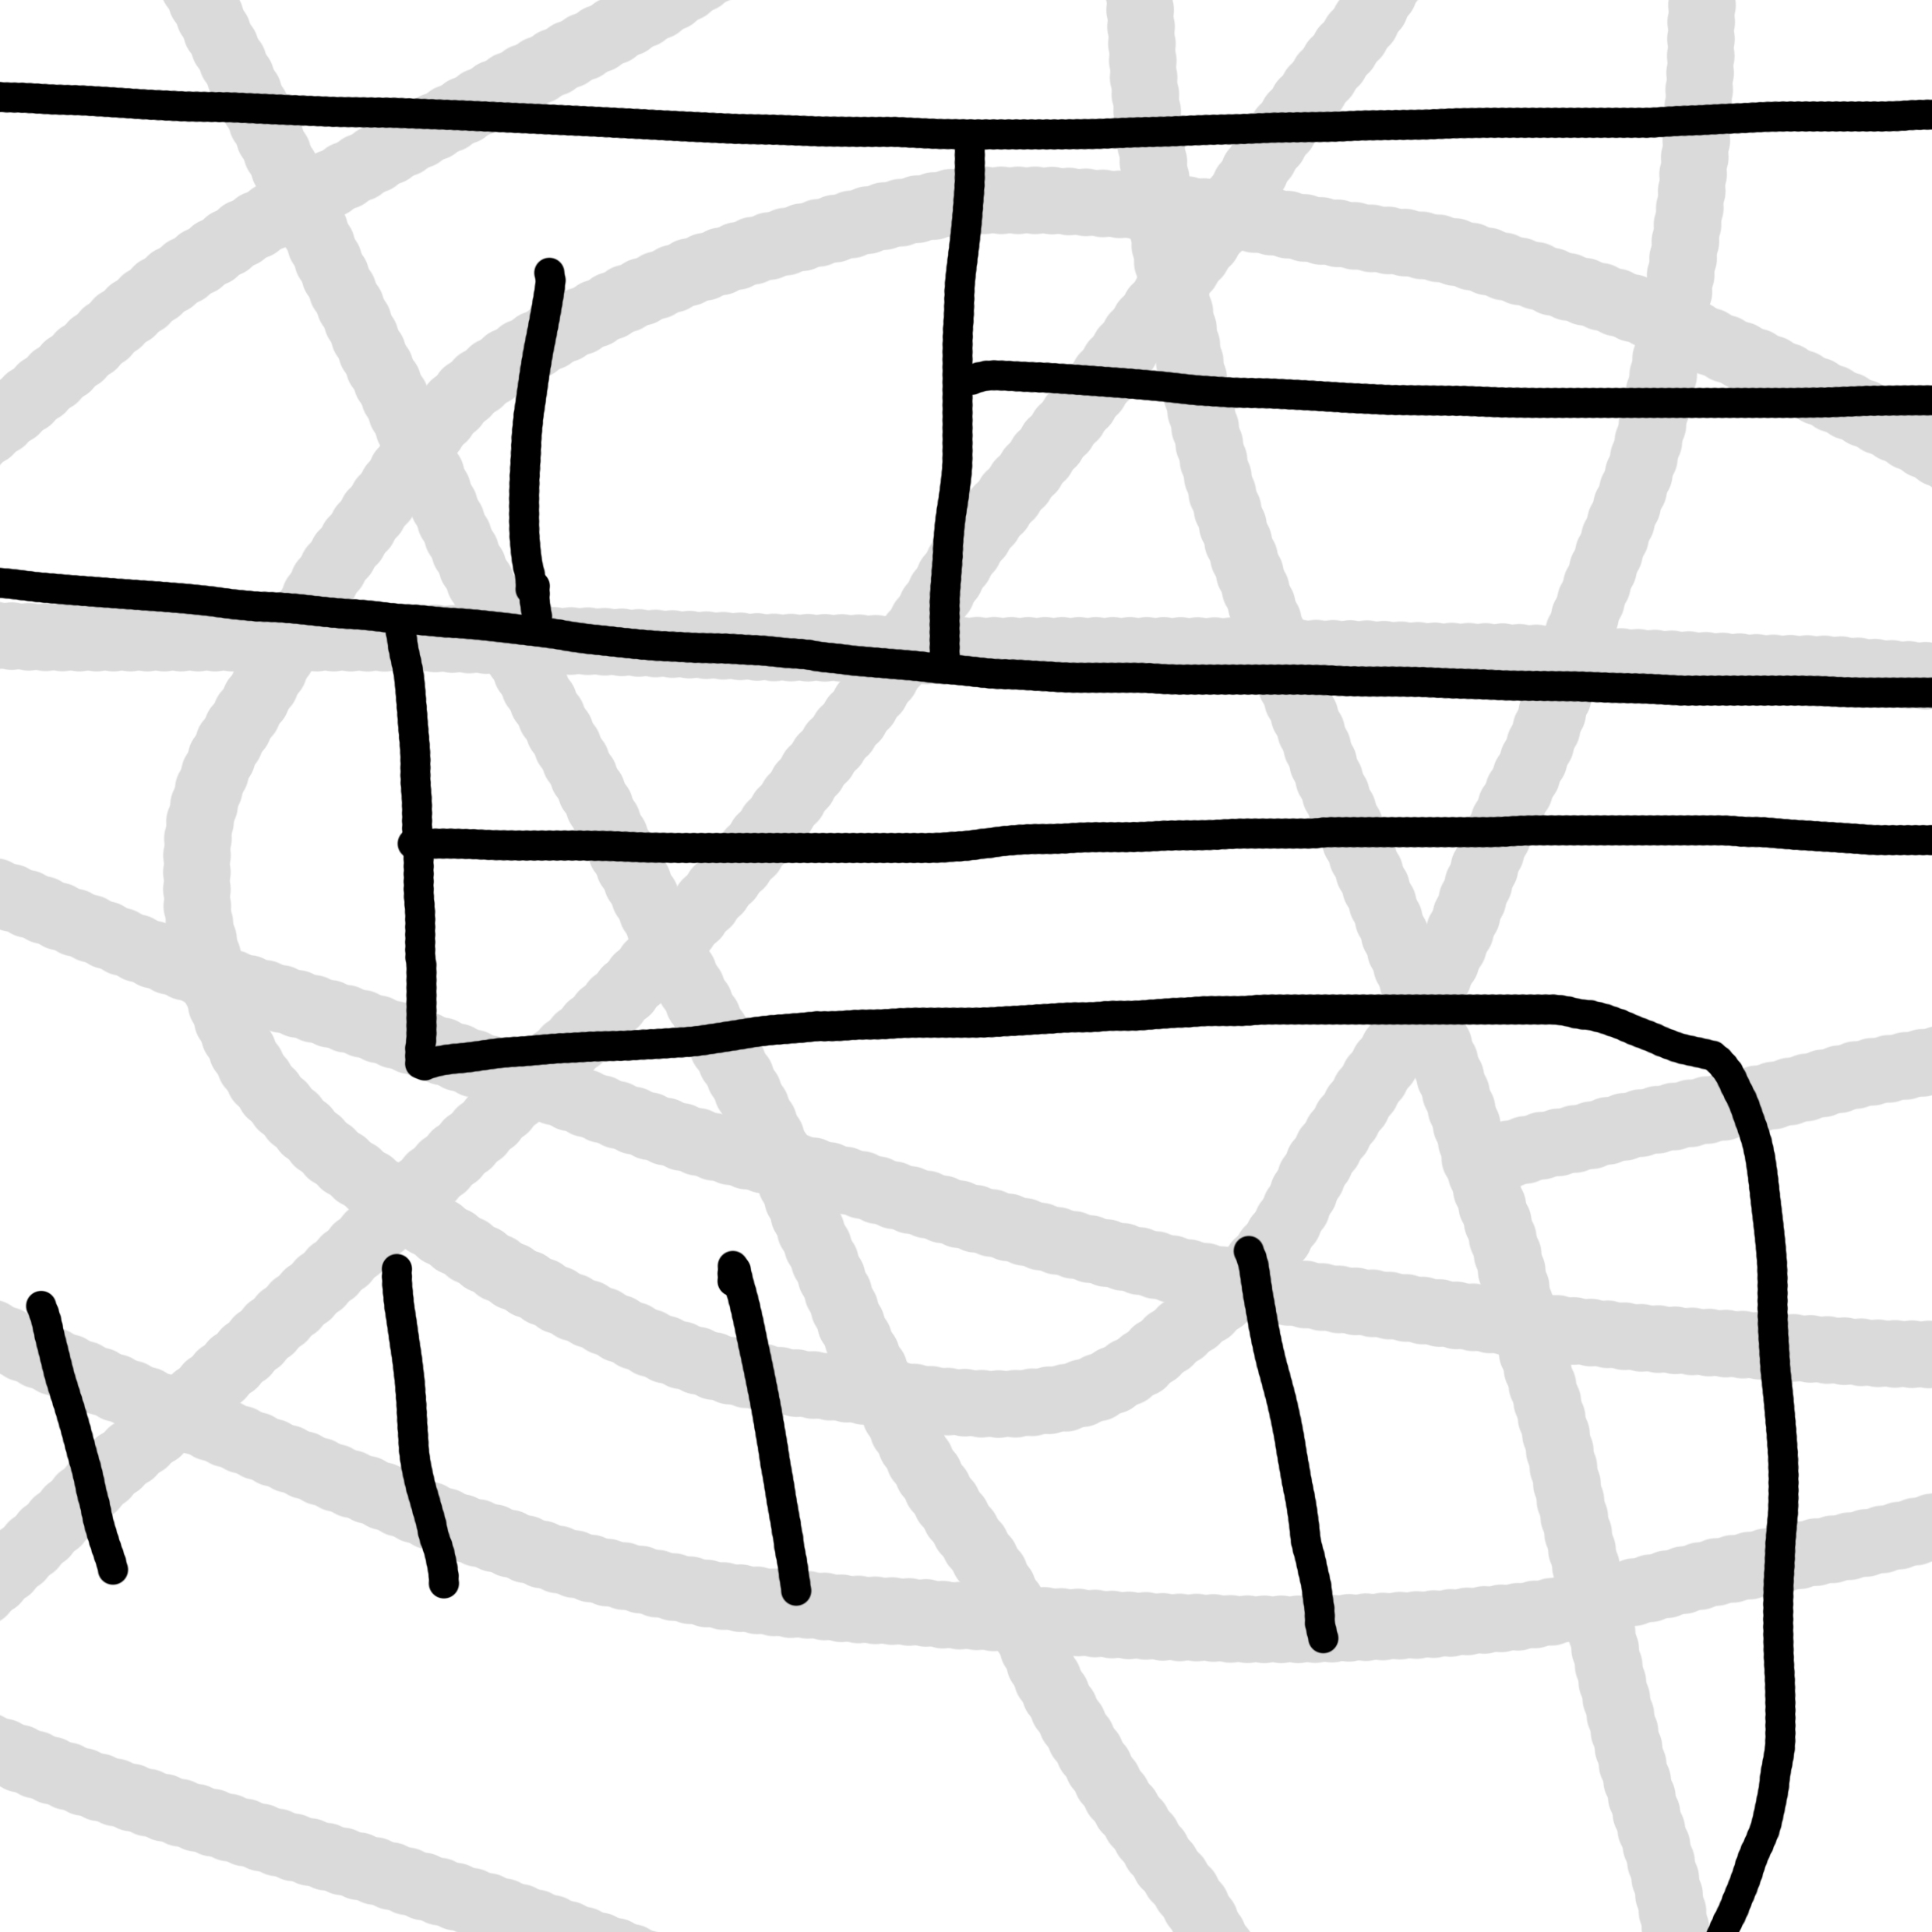
\includegraphics[scale=0.2]{img/user_task_puzzle1.jpg}\hspace{1cm}

\includegraphics[scale=0.2]{img/user_task_puzzle2.jpg}
\caption{left: the puzzle used in face-to-face collaboration; right: the puzzle used in CSCW}
\label{fig:field_task1}
\end{figure}

Task 2, \textit{layout design}.

Face-to-face instruction: Ming is a prospective 25-year-old male master student, he is moving to his new accommodation and need to layout his corridor room with the following staff. Please design his bedroom layout with your partner in the given rectangular space.

CSCW instruction: Cai is a 30-year-old lady, she is moving to her new place due to work transition and would only stay here for half a year. Please design her bedroom layout with your partner in the given rectangular space.

The room layout design elements are shown in figure \ref{fig:field_task2}. \\

\begin{figure}[h!]
\centering
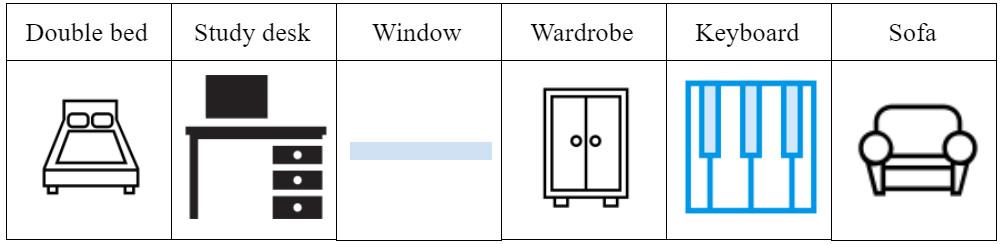
\includegraphics[scale=1]{img/user_task2_f2f.PNG}\\
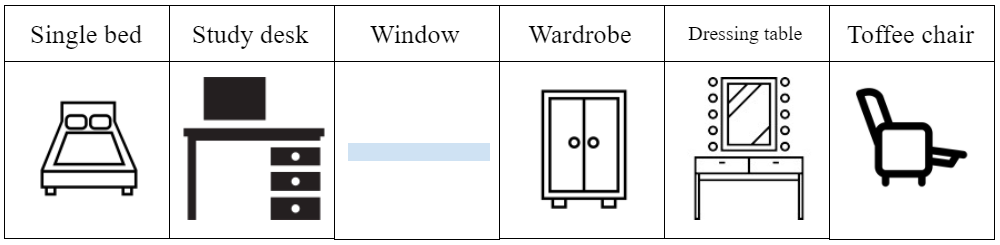
\includegraphics[scale=1]{img/user_task2_CSCW.PNG}
\caption{Top: the furnitures used in face-to-face collaboration; bottom: the furnitures used in CSCW}
\label{fig:field_task2}
\end{figure}

Task 3, \textit{storyboard design based on previous room layout}.

Face-to-face instruction: Please tell a story describing how Ming does in his bedroom in the evening of an average day using the given six-rectangle space.

CSCW instruction: Please tell a story describing how Cai does in her bedroom in the morning of an average day using the given six-rectangle space.


\section{Evaluation user tasks}
\label{appdx:evaluationtask}

We designed two tasks for evaluation. Task requirement and detailed instructions given to test subjects are the follows, the graphic illustration we used are shown in the figure \ref{fig:eva_task}.\\

Task 1, \textit{puzzle piece moving}.

Imagine you are working with your remote collaborator. Please ask him to move the top right piece into bottom left corner.\\

Task 2, \textit{layout design}.

Imagine you are working with your remote collaborator. The sofa is not placed in the room currently. Please express your sofa layout idea to your collaborator, describe which position the sofa should be positioned, and which direction it should take.

\begin{figure}[h!]
\centering
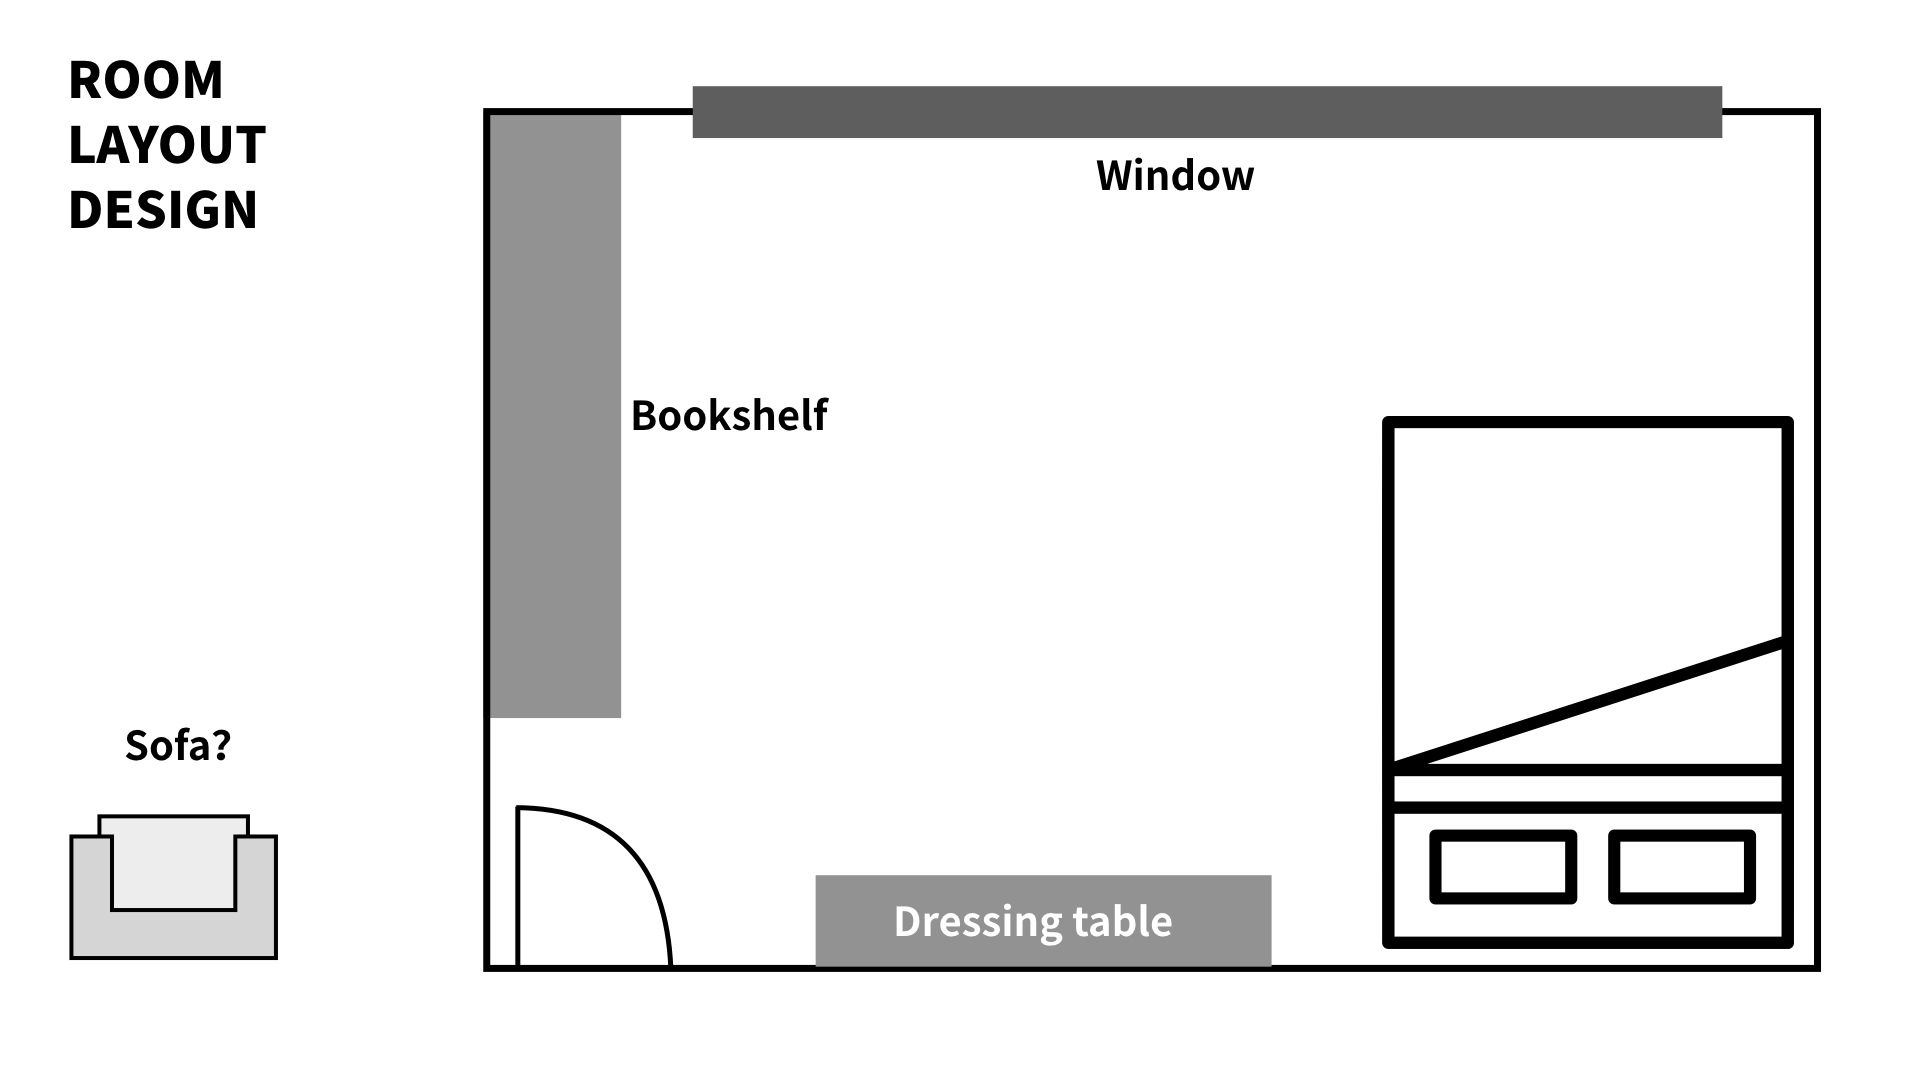
\includegraphics[scale=0.12]{img/eva_task1.jpg}
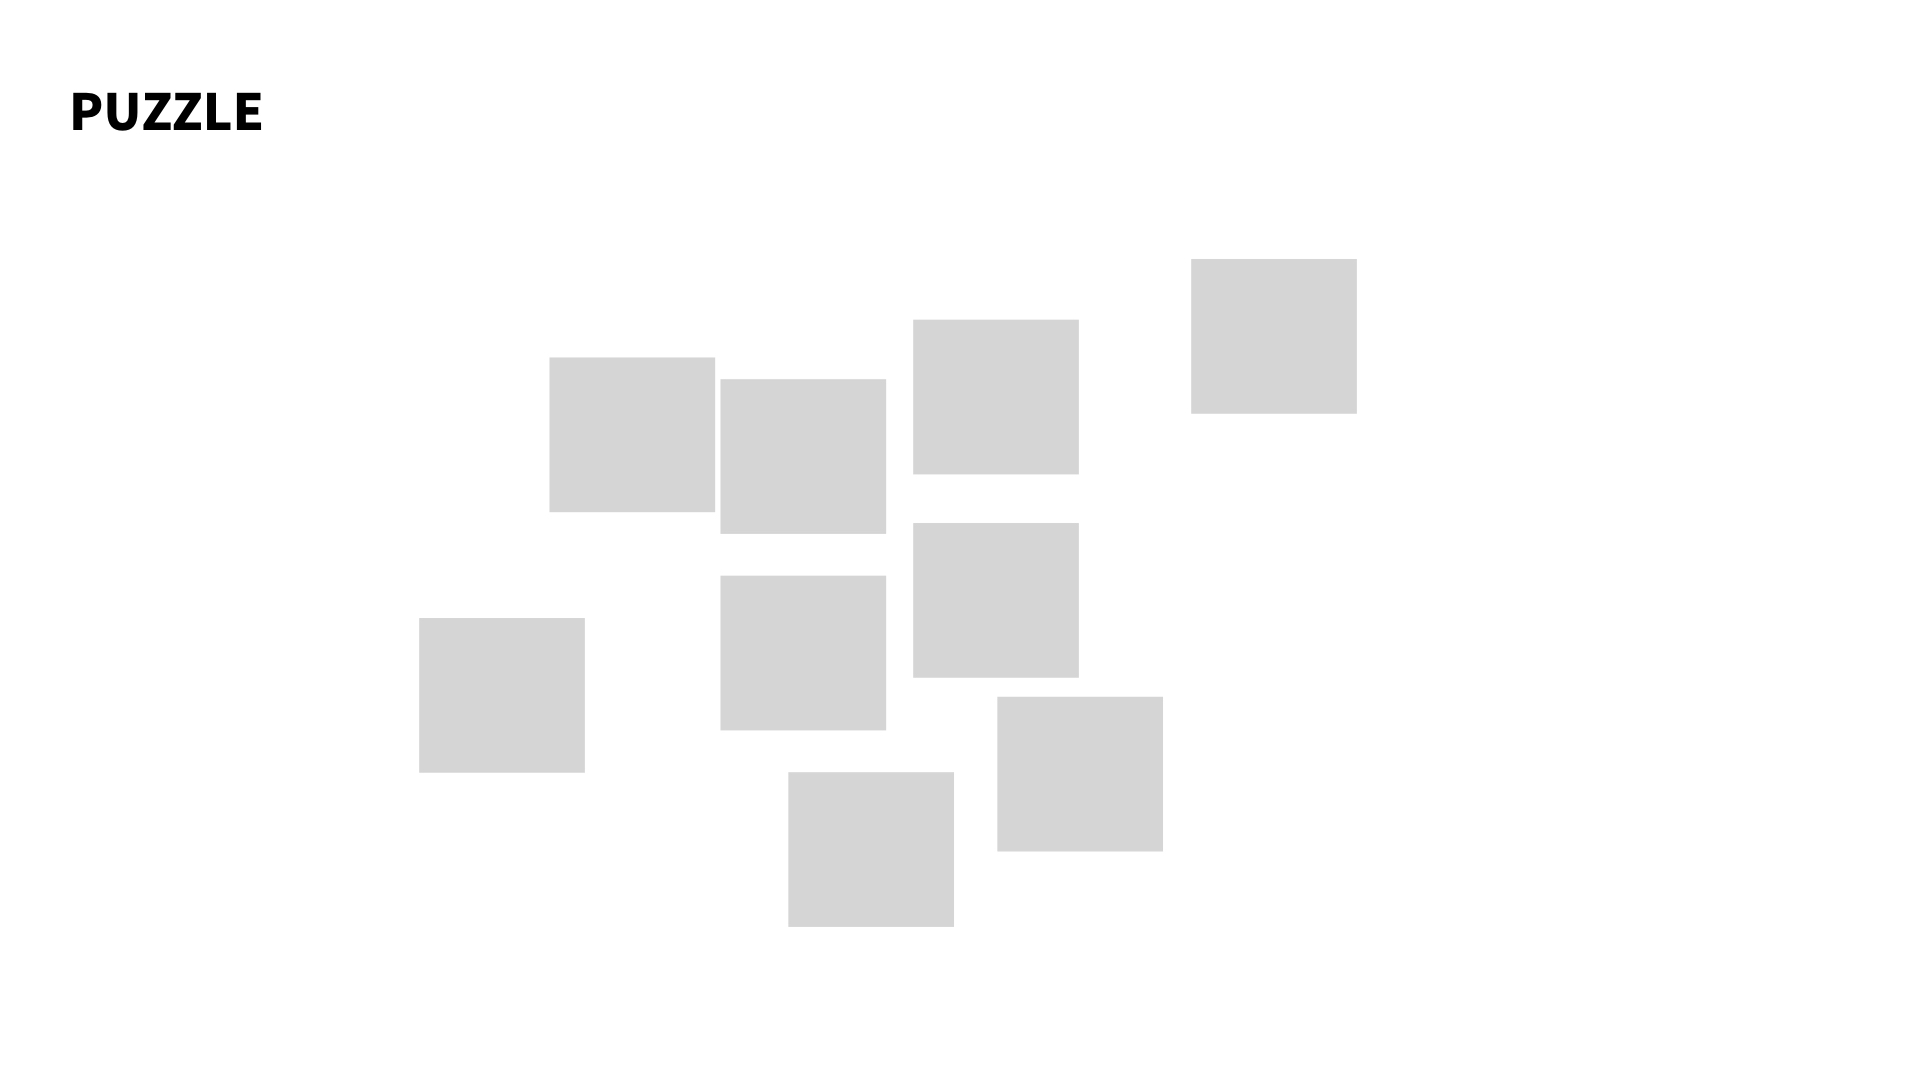
\includegraphics[scale=0.12]{img/eva_task2.jpg}
\caption{Evaluation tasks graphic illustraions}\label{fig:eva_task}
\end{figure}

\end{document}
